\subsection{Supplementary Figures}

\begin{figure}[htbp]
    \centering
    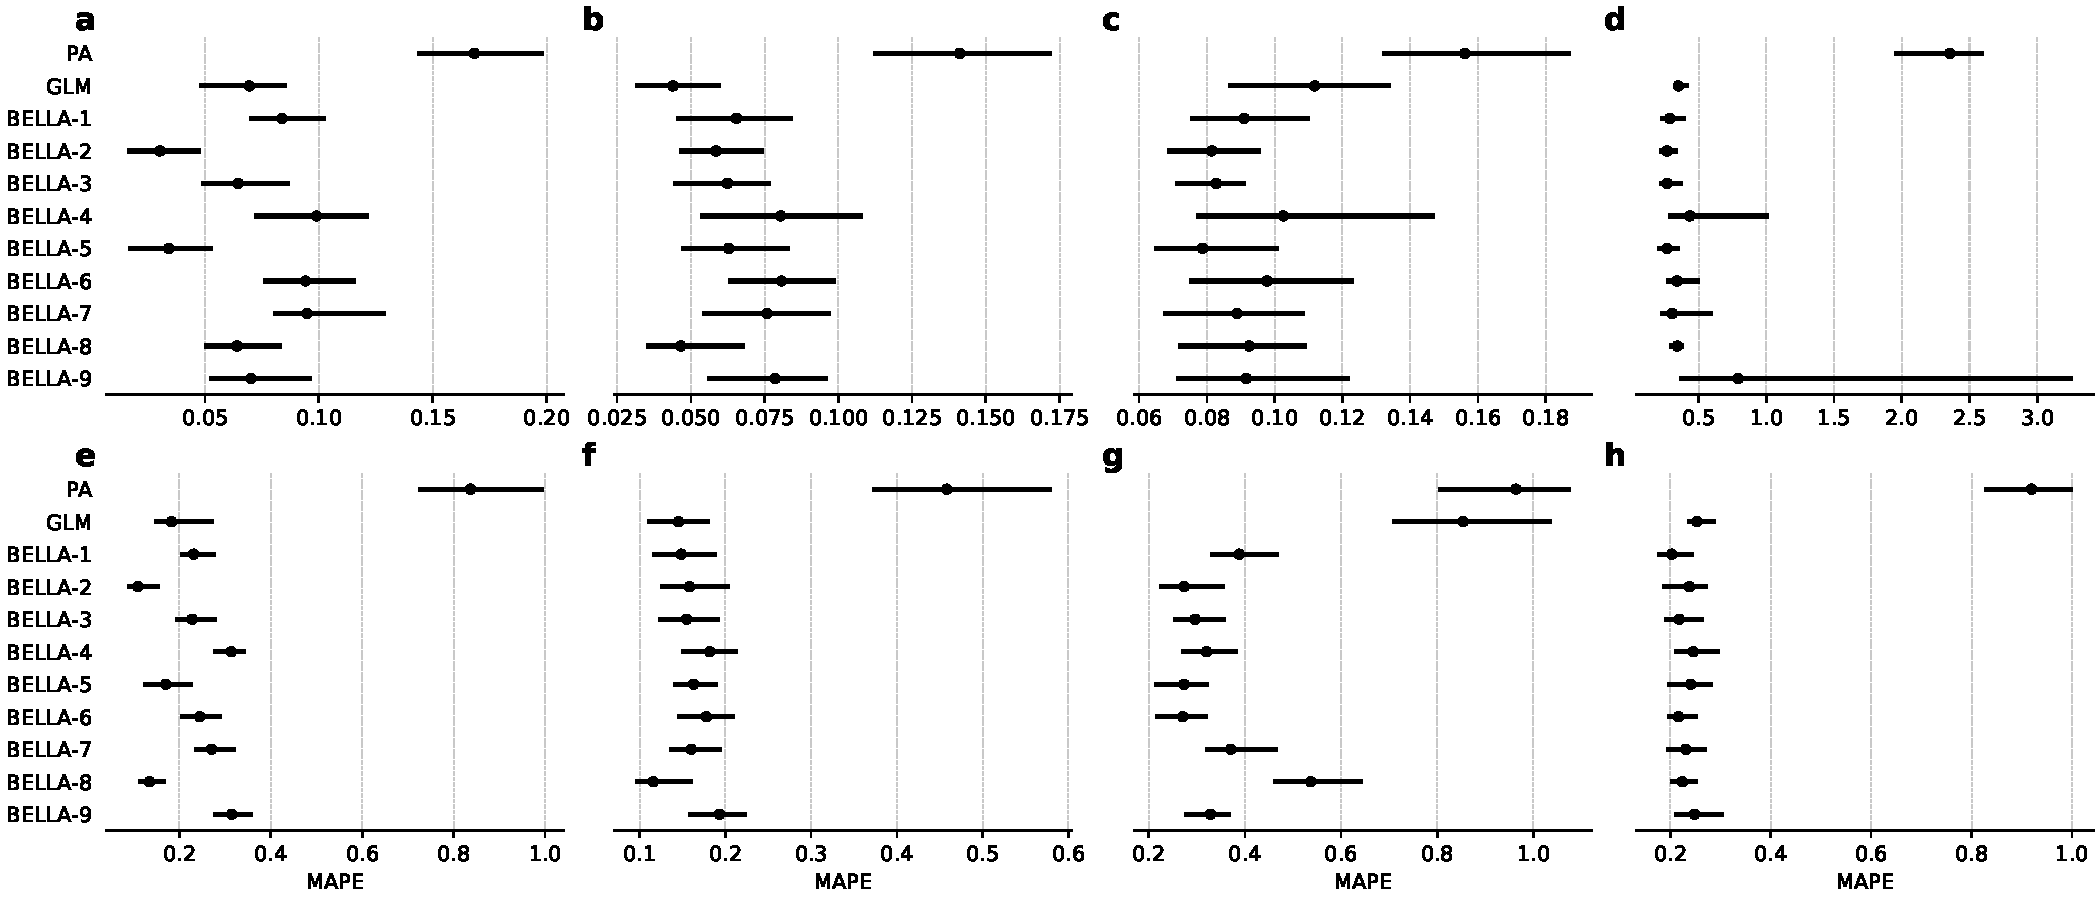
\includegraphics[width=1\textwidth]{figures/metrics/mape.pdf}
    \caption{Cross-scenario comparison of mean absolute percentage error (MAPE) for all fitted models across 100 simulation replicates. Each panel corresponds to one simulation scenario: (a) \texttt{Epi-1}, (b) \texttt{Epi-2}, (c) \texttt{Epi-3}, (d) \texttt{Epi-4}, (e) \texttt{FBD-1}, (f) \texttt{FBD-2}, (g) \texttt{FBD-3}, and (h) \texttt{FBD-4}. The y-axis lists the predictor-agnostic (PA), GLM, and BELLA configurations. For each model, the point gives the median MAPE across simulation replicates after averaging over the target parameters, and the horizontal segment gives the 50\% interquartile range; smaller values indicate more accurate posterior medians.}%
    \label{fig:metrics:mape}
\end{figure}

\begin{figure}[htbp]
    \centering
    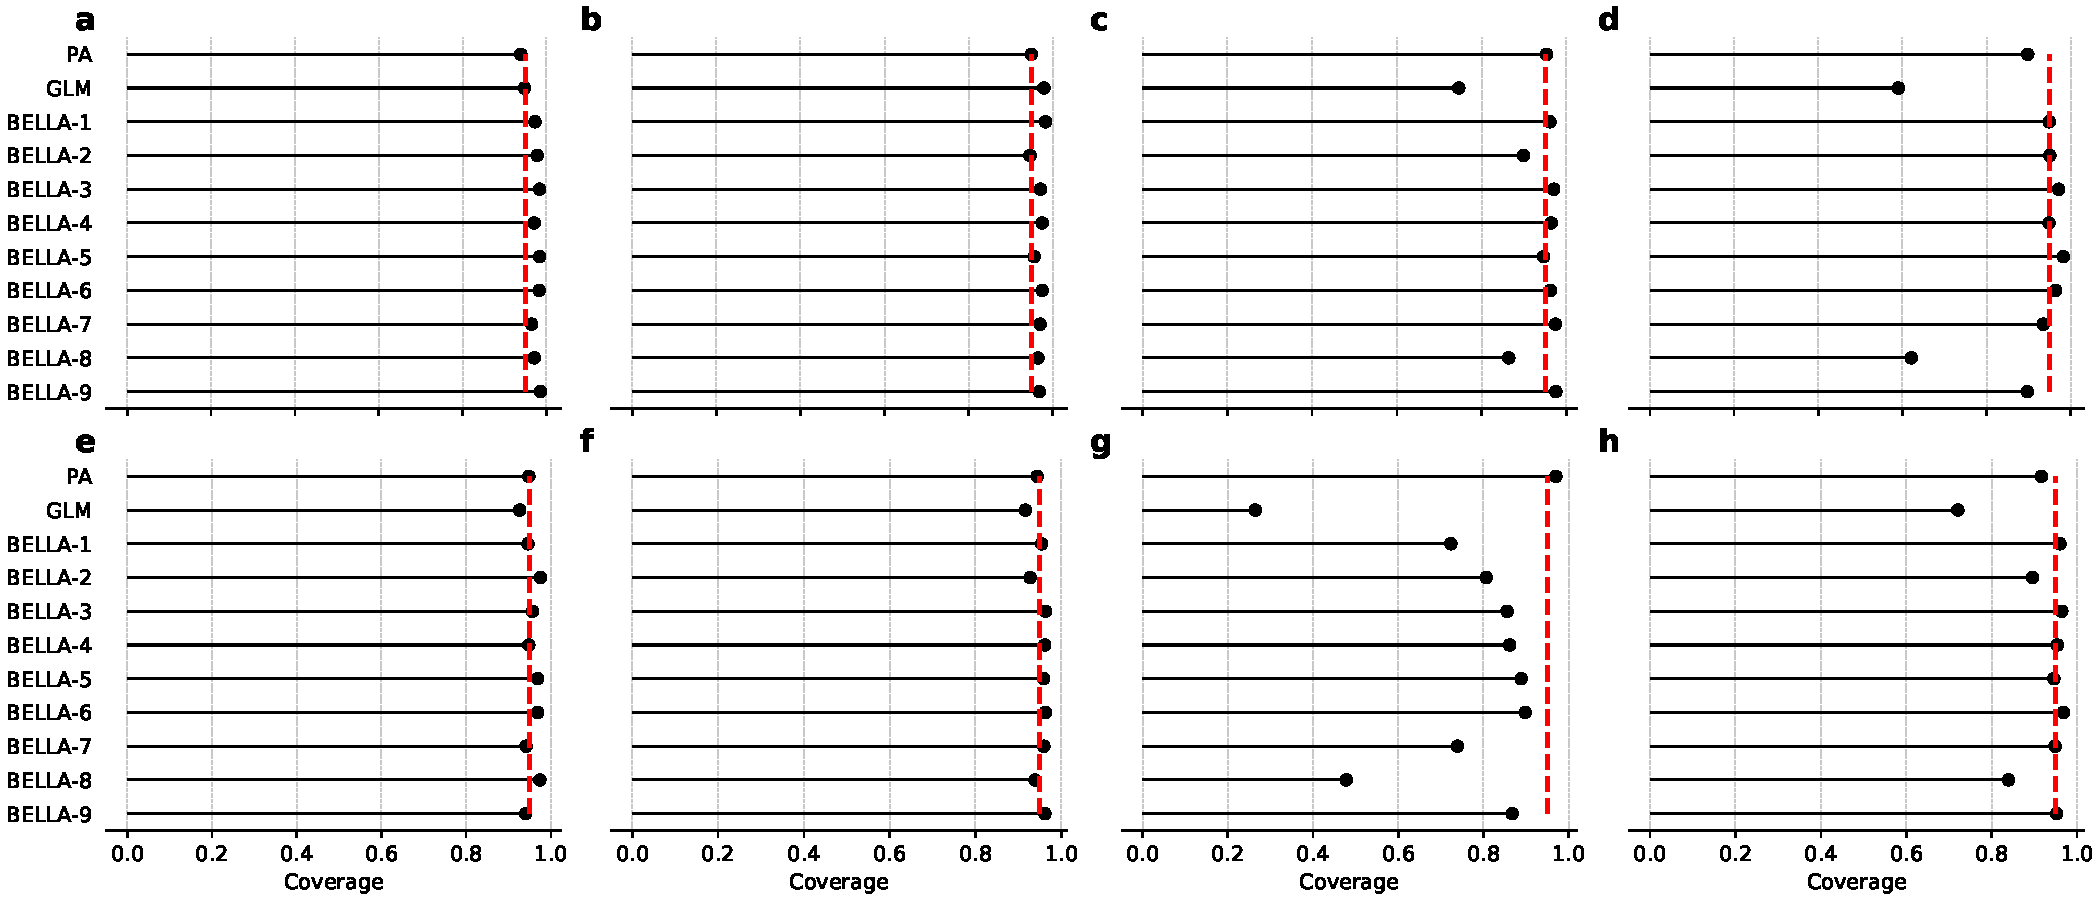
\includegraphics[width=1\textwidth]{figures/metrics/coverage.pdf}
    \caption{Cross-scenario comparison of empirical 95\% credible-interval coverage across 100 simulation replicates. Each panel corresponds to one simulation scenario: (a) \texttt{Epi-1}, (b) \texttt{Epi-2}, (c) \texttt{Epi-3}, (d) \texttt{Epi-4}, (e) \texttt{FBD-1}, (f) \texttt{FBD-2}, (g) \texttt{FBD-3}, and (h) \texttt{FBD-4}. The y-axis lists the predictor-agnostic (PA), GLM, and BELLA configurations. For each model, the point reports the target-averaged fraction of true simulated parameter values contained in the posterior interval bounds across simulation replicates; values closer to nominal coverage (dashed red line) indicate better uncertainty calibration.}%
    \label{fig:metrics:coverage}
\end{figure}

\begin{figure}[htbp]
    \centering
    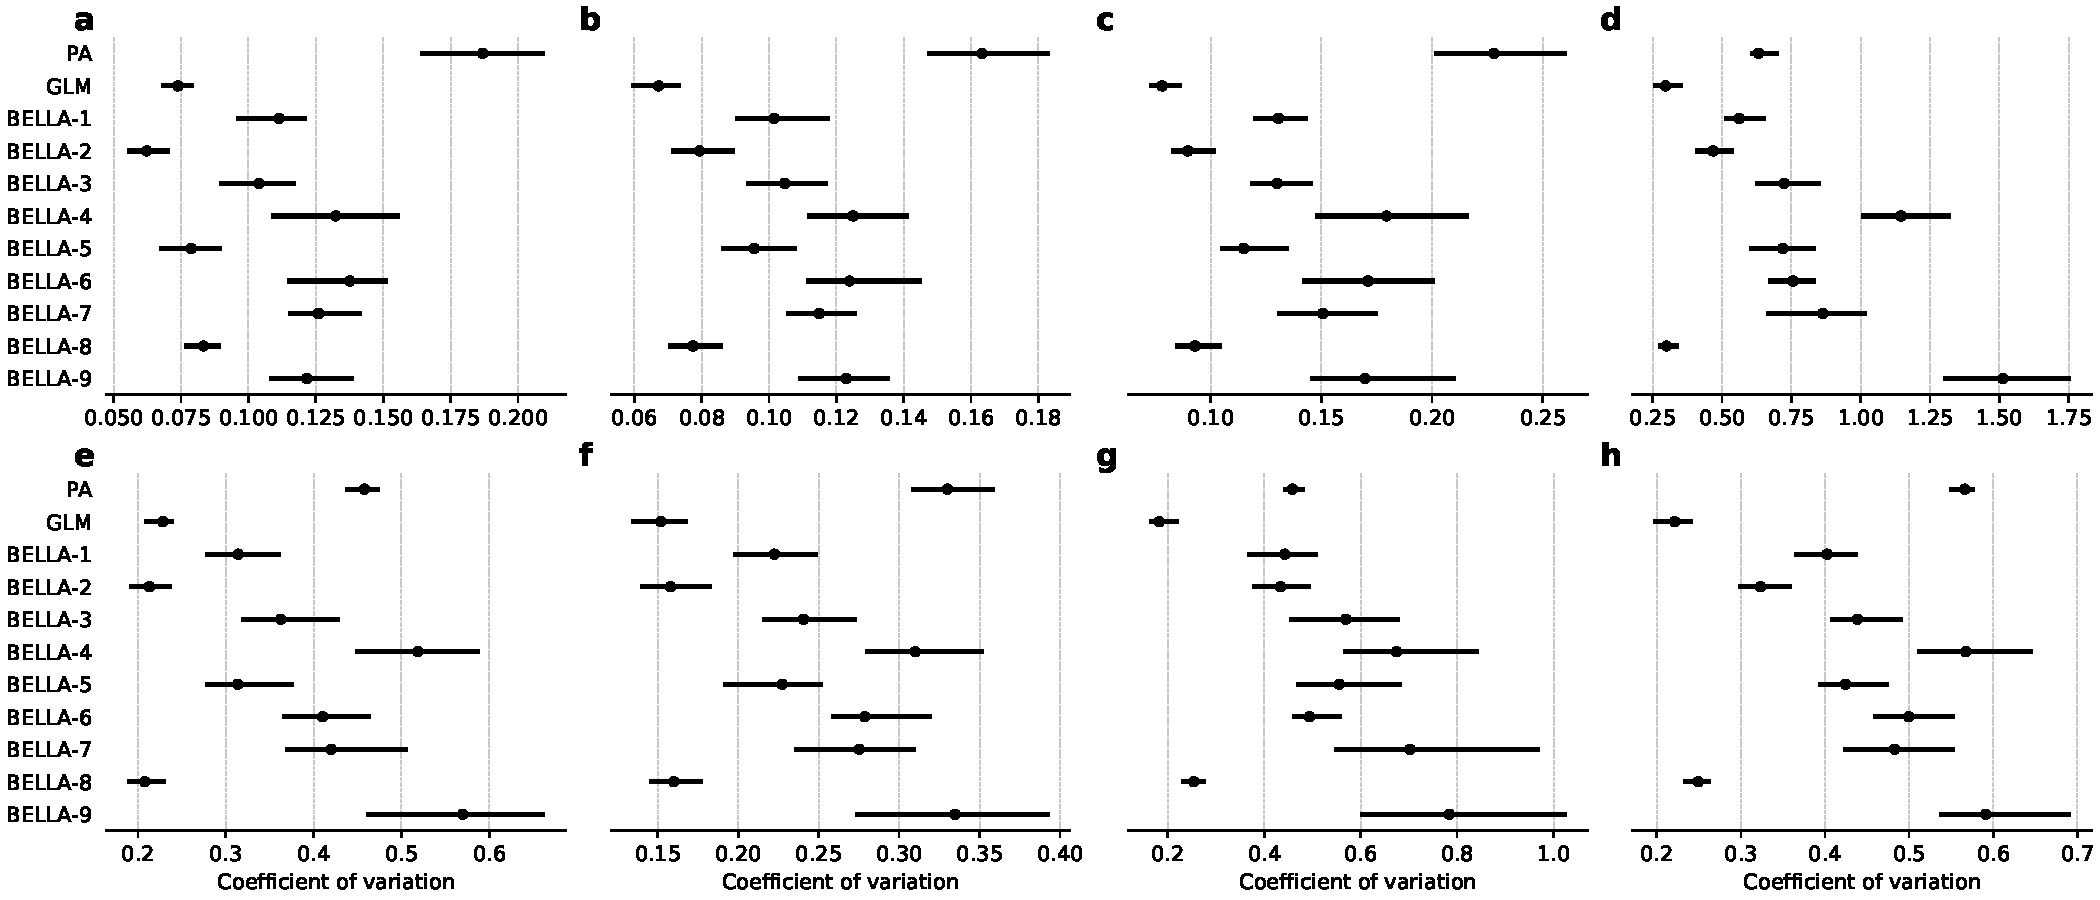
\includegraphics[width=1\textwidth]{figures/metrics/cv.pdf}
    \caption{Cross-scenario comparison of posterior coefficient of variation across 100 simulation replicates. Each panel corresponds to one simulation scenario: (a) \texttt{Epi-1}, (b) \texttt{Epi-2}, (c) \texttt{Epi-3}, (d) \texttt{Epi-4}, (e) \texttt{FBD-1}, (f) \texttt{FBD-2}, (g) \texttt{FBD-3}, and (h) \texttt{FBD-4}. The y-axis lists the predictor-agnostic (PA), GLM, and BELLA configurations. For each model, the point gives the median coefficient of variation across simulation replicates after averaging over target parameters, and the horizontal segment gives the 50\% interquartile range; smaller values indicate more concentrated posterior estimates relative to their posterior means.}%
    \label{fig:metrics:cv}
\end{figure}

\begin{figure}[htbp]
    \centering
    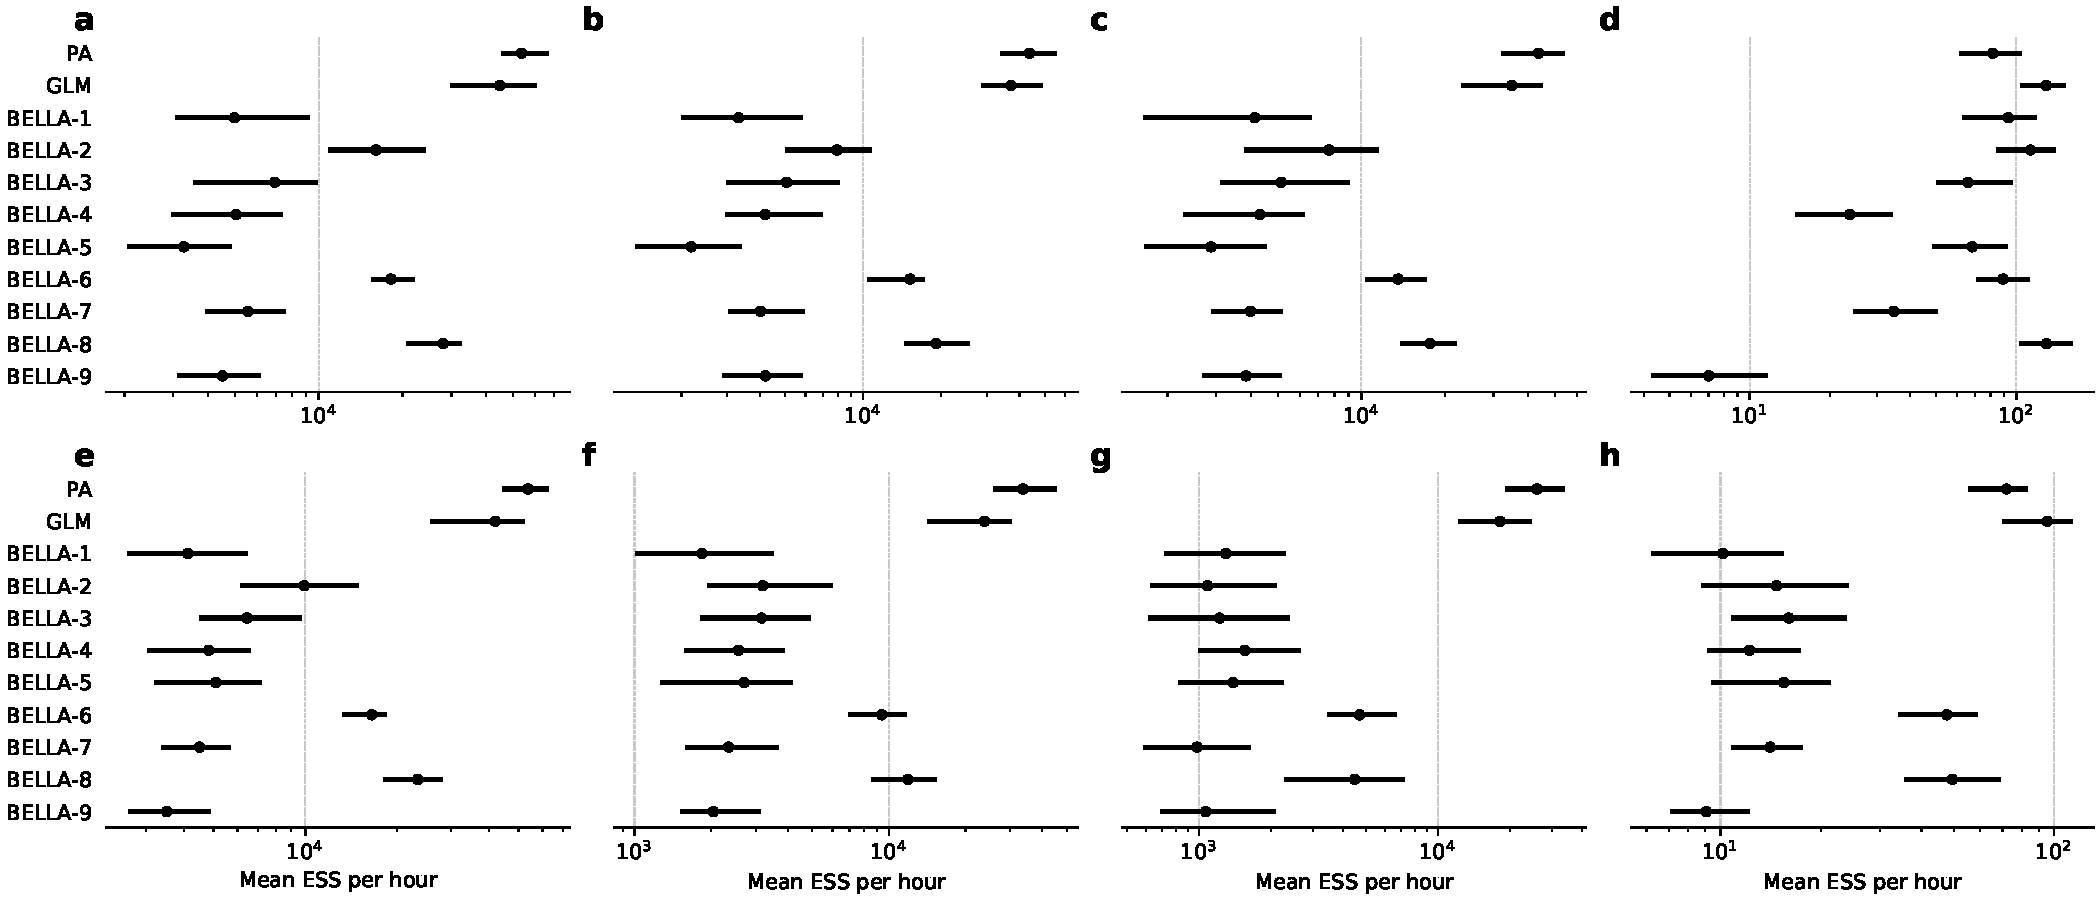
\includegraphics[width=1\textwidth]{figures/metrics/mean_ess_per_hour.pdf}
    \caption{Cross-scenario comparison of mean effective sample size (ESS) per hour across 100 simulation replicates. Each panel corresponds to one simulation scenario: (a) \texttt{Epi-1}, (b) \texttt{Epi-2}, (c) \texttt{Epi-3}, (d) \texttt{Epi-4}, (e) \texttt{FBD-1}, (f) \texttt{FBD-2}, (g) \texttt{FBD-3}, and (h) \texttt{FBD-4}. The y-axis lists the predictor-agnostic (PA), GLM, and BELLA configurations. For each model, the point gives the median target-averaged ESS per hour across simulation replicates, and the horizontal segment gives the 50\% interquartile range; the x-axis is logarithmic, and larger values indicate greater sampling efficiency.}%
    \label{fig:metrics:mean_ess_per_hour}
\end{figure}

\begin{figure}[htbp]
    \centering
    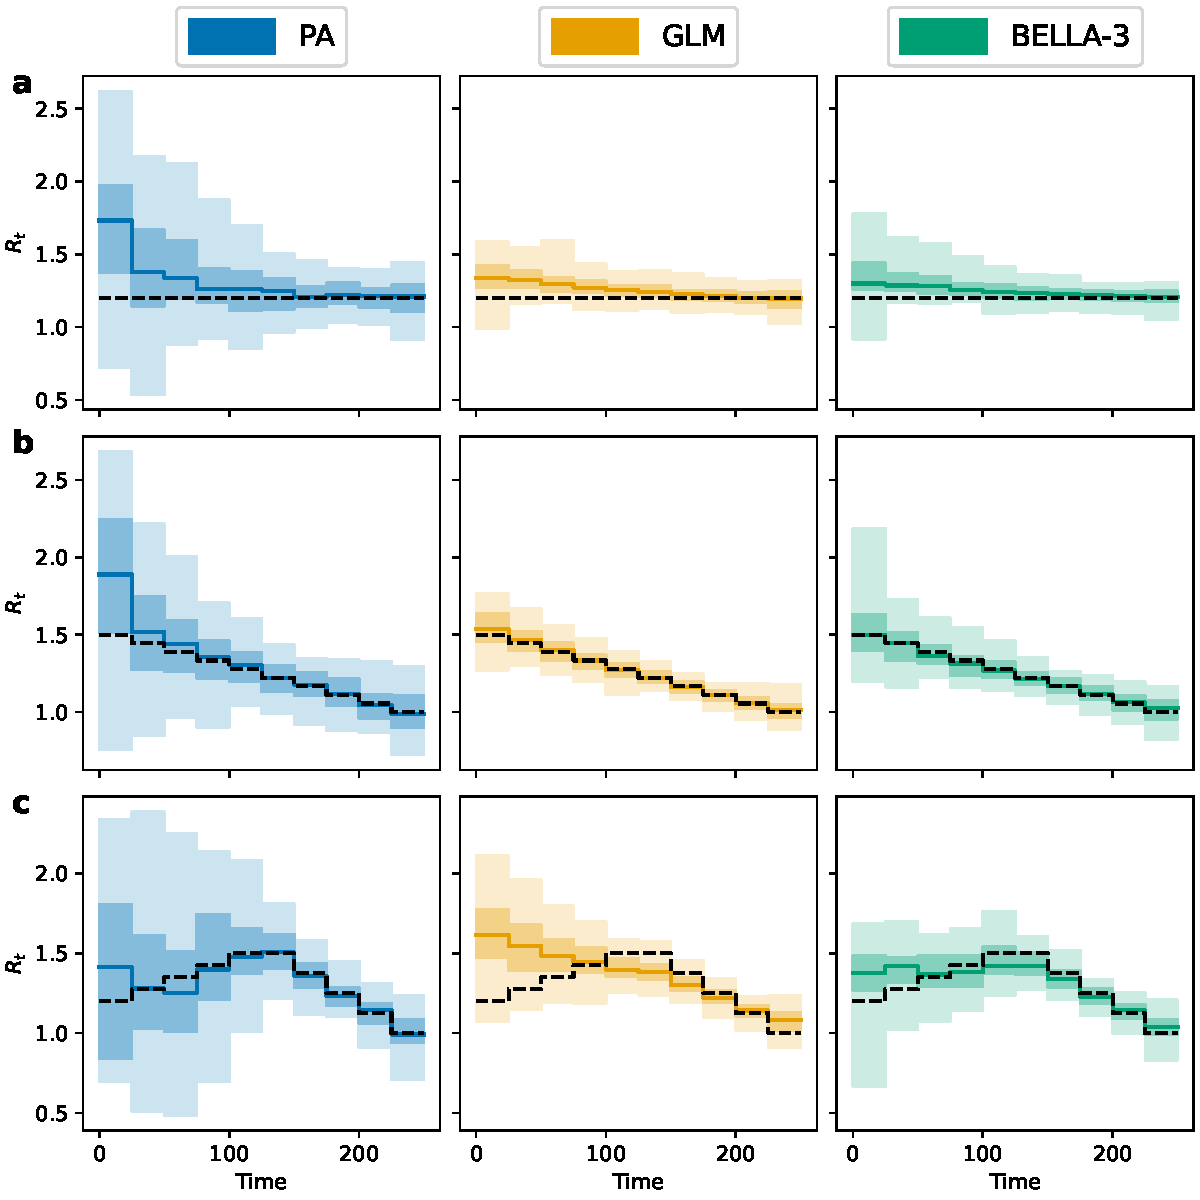
\includegraphics[width=1\textwidth]{figures/epi-skyline/ribbons.pdf}
    \caption{Reconstruction of the epidemiological skyline $R_t$ trajectories by predictor-agnostic (PA), GLM, and the reference BELLA model across 100 simulation replicates. Rows correspond to simulation scenarios: (a) \texttt{Epi-1} with constant $R_t$, (b) \texttt{Epi-2} with monotonically decreasing $R_t$, and (c) \texttt{Epi-3} with an increase followed by a decrease. Columns correspond to predictor-agnostic (PA), GLM, and \texttt{BELLA-3}. In each panel, the solid line shows the posterior median trajectory across simulation replicates, while the colored ribbons summarize its distribution, with the darker ribbon showing the 50\% interquantile range and the lighter ribbon showing the 95\% interquantile range; the black dashed line shows the true simulated $R_t$ trajector.}%
    \label{fig:epi-skyline:ribbons}
\end{figure}

\begin{figure}[htbp]
    \centering
    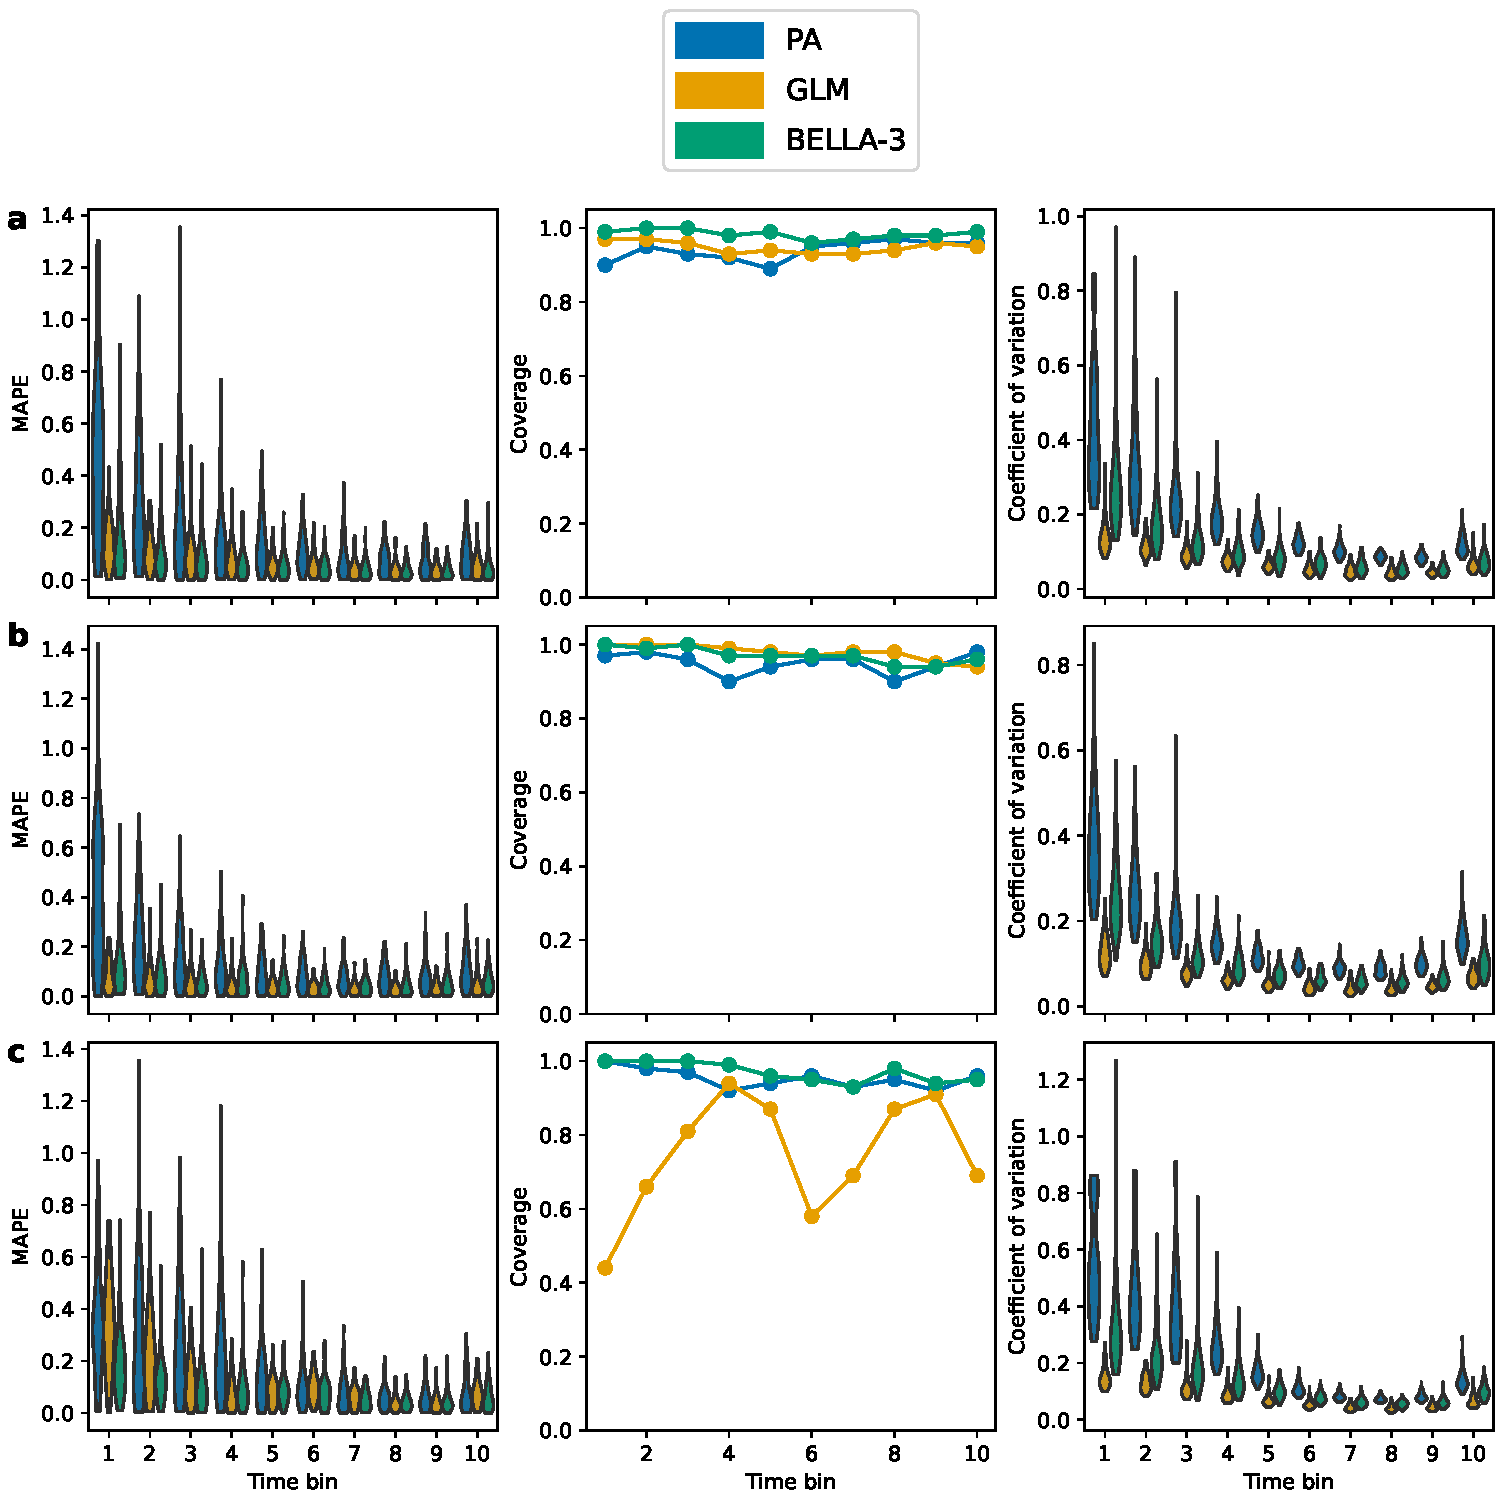
\includegraphics[width=1\textwidth]{figures/epi-skyline/metrics.pdf}
    \caption{Time-resolved accuracy and uncertainty diagnostics for the epidemiological skyline simulations across 100 simulation replicates. Rows correspond to simulation scenarios: (a) \texttt{Epi-1}, (b) \texttt{Epi-2}, and (c) \texttt{Epi-3}. Columns show mean absolute percentage error (MAPE), empirical coverage, and coefficient of variation by time bin. Colored distributions or lines compare predictor-agnostic (PA), GLM, and \texttt{BELLA-3}; MAPE and coefficient of variation are evaluated per replicate, whereas coverage is evaluated as the fraction of intervals containing the true $R_t$ value in each time bin.}%
    \label{fig:epi-skyline:metrics}
\end{figure}

\begin{figure}[htbp]
    \centering
    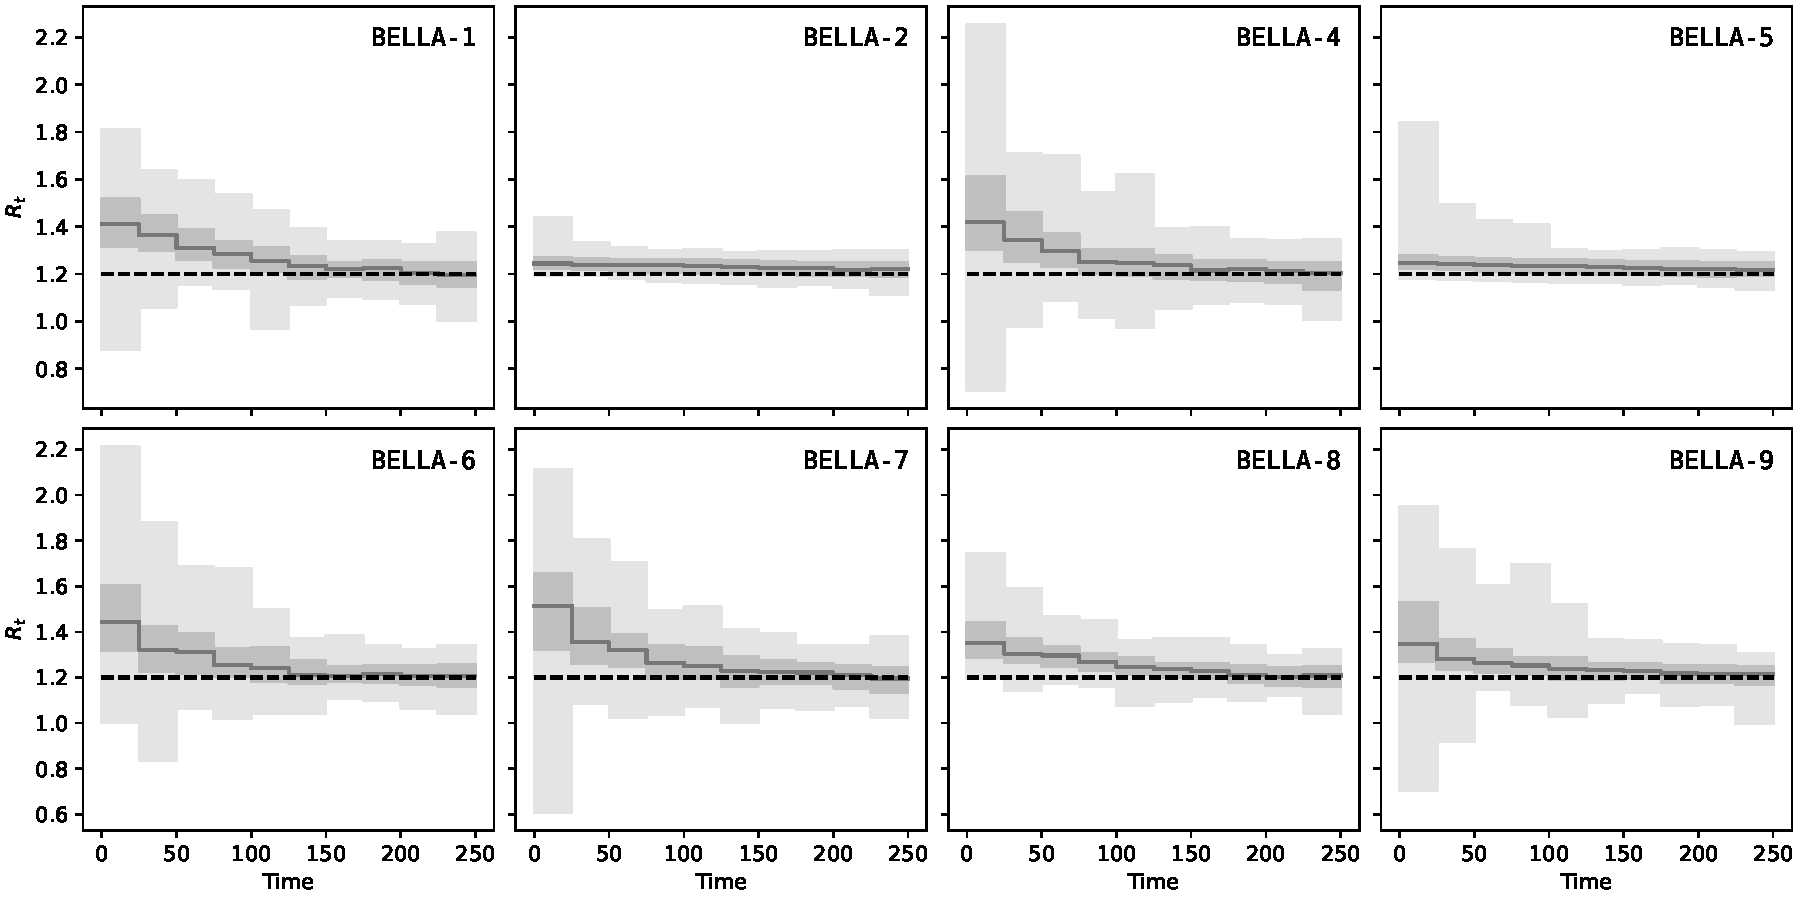
\includegraphics[width=1\textwidth]{figures/epi-skyline/sensitivity/epi-skyline_1.pdf}
    \caption{Sensitivity of BELLA architecture choices for the constant epidemiological skyline scenario (\texttt{Epi-1}) across 100 simulation replicates. In each panel, the solid line shows the posterior median $R_t$ trajectory across simulation replicates, while the colored ribbons summarize its distribution, with the darker ribbon showing the 50\% interquantile range and the lighter ribbon showing the 95\% interquantile range; the black dashed line shows the true simulated $R_t$ trajectory.}%
    \label{fig:epi-skyline:sensitivity:epi-skyline_1}
\end{figure}

\begin{figure}[htbp]
    \centering
    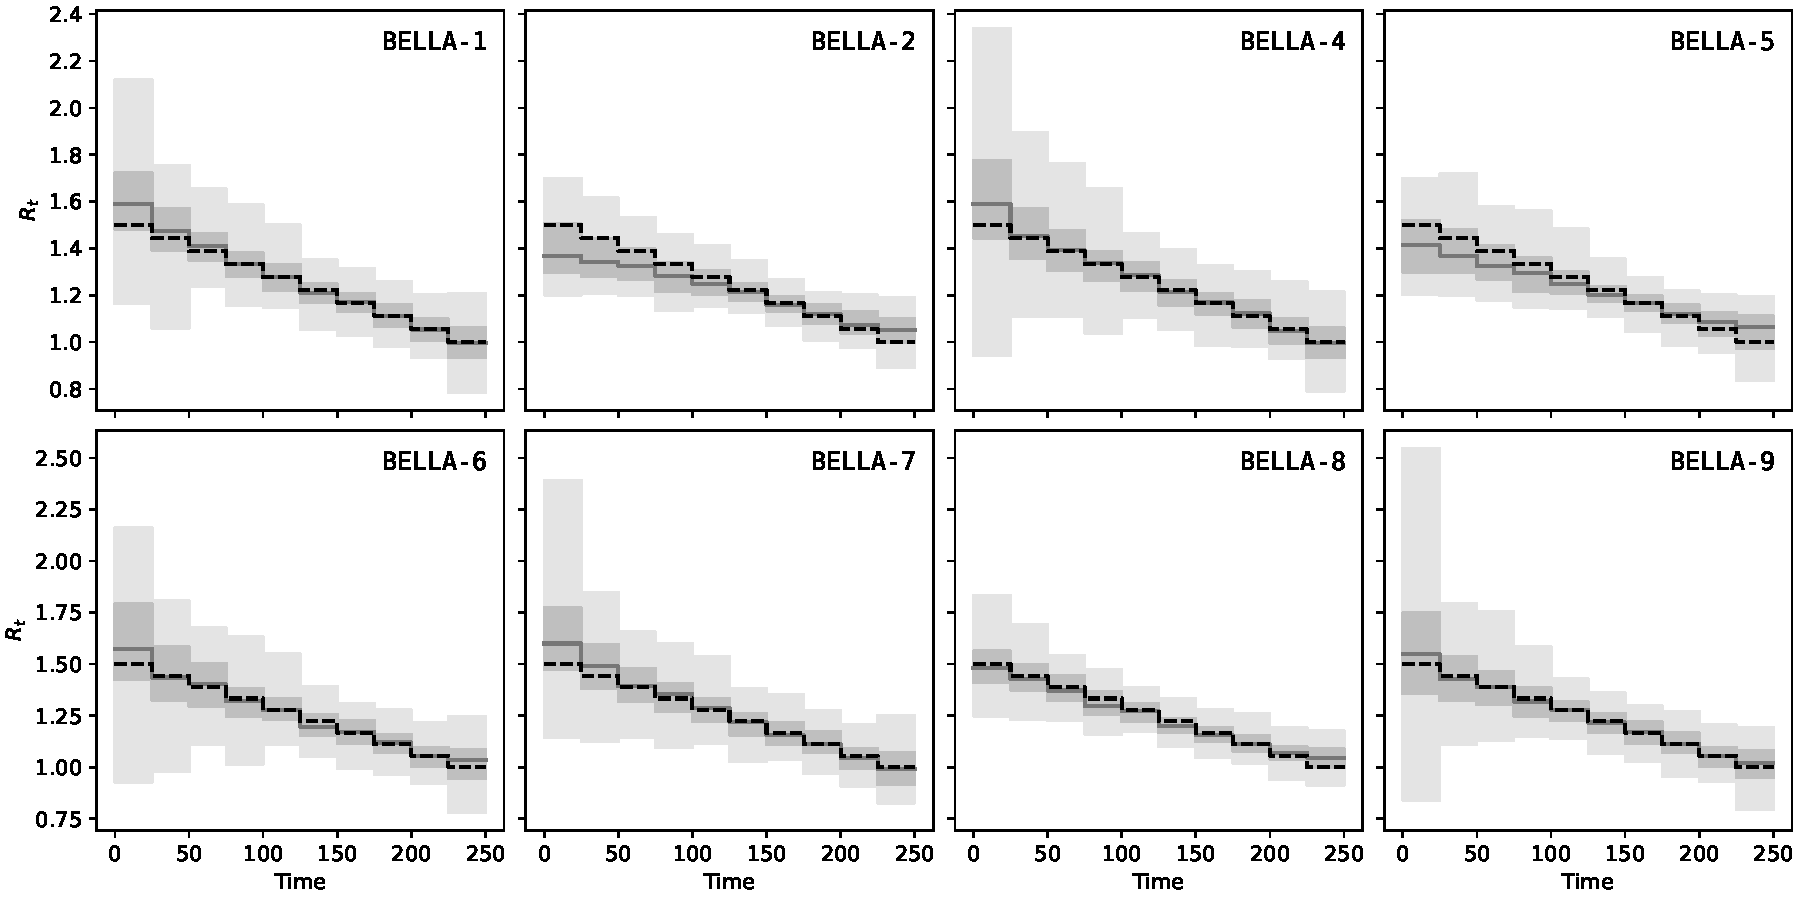
\includegraphics[width=1\textwidth]{figures/epi-skyline/sensitivity/epi-skyline_2.pdf}
    \caption{Sensitivity of BELLA architecture choices for the constant epidemiological skyline scenario (\texttt{Epi-2}) across 100 simulation replicates. In each panel, the solid line shows the posterior median $R_t$ trajectory across simulation replicates, while the colored ribbons summarize its distribution, with the darker ribbon showing the 50\% interquantile range and the lighter ribbon showing the 95\% interquantile range; the black dashed line shows the true simulated $R_t$ trajectory.}%
    \label{fig:epi-skyline:sensitivity:epi-skyline_2}
\end{figure}

\begin{figure}[htbp]
    \centering
    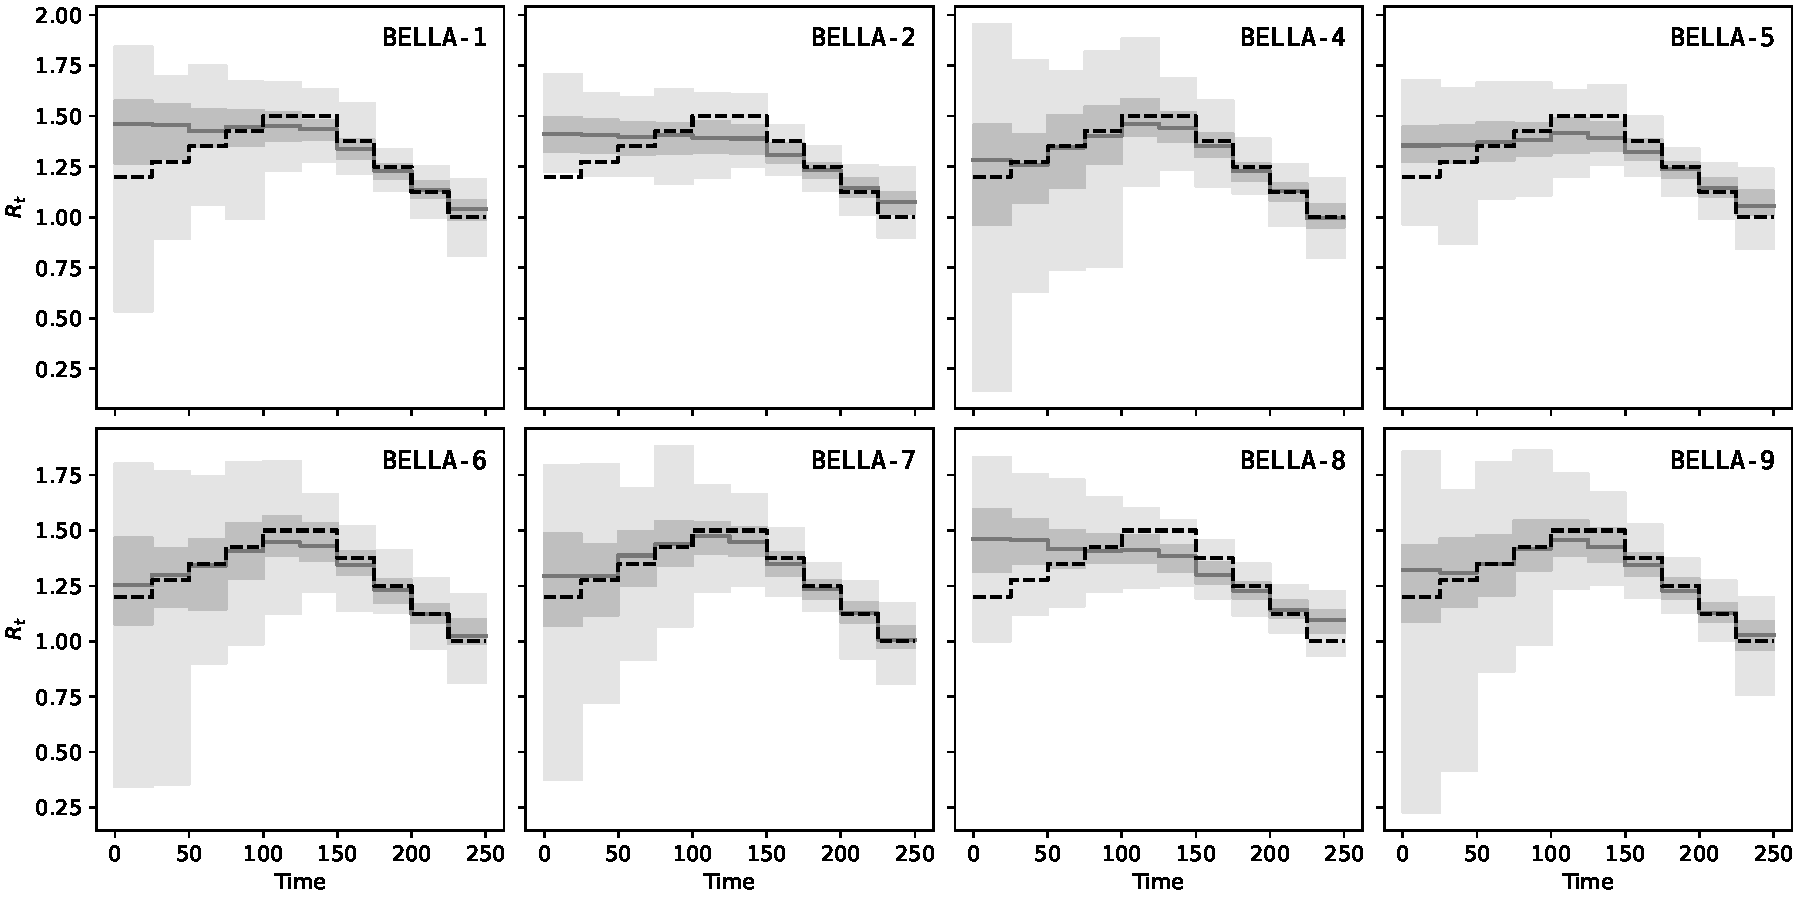
\includegraphics[width=1\textwidth]{figures/epi-skyline/sensitivity/epi-skyline_3.pdf}
    \caption{Sensitivity of BELLA architecture choices for the constant epidemiological skyline scenario (\texttt{Epi-3}) across 100 simulation replicates. In each panel, the solid line shows the posterior median $R_t$ trajectory across simulation replicates, while the colored ribbons summarize its distribution, with the darker ribbon showing the 50\% interquantile range and the lighter ribbon showing the 95\% interquantile range; the black dashed line shows the true simulated $R_t$ trajectory.}%
    \label{fig:epi-skyline:sensitivity:epi-skyline_3}
\end{figure}

\begin{figure}[htbp]
    \centering
    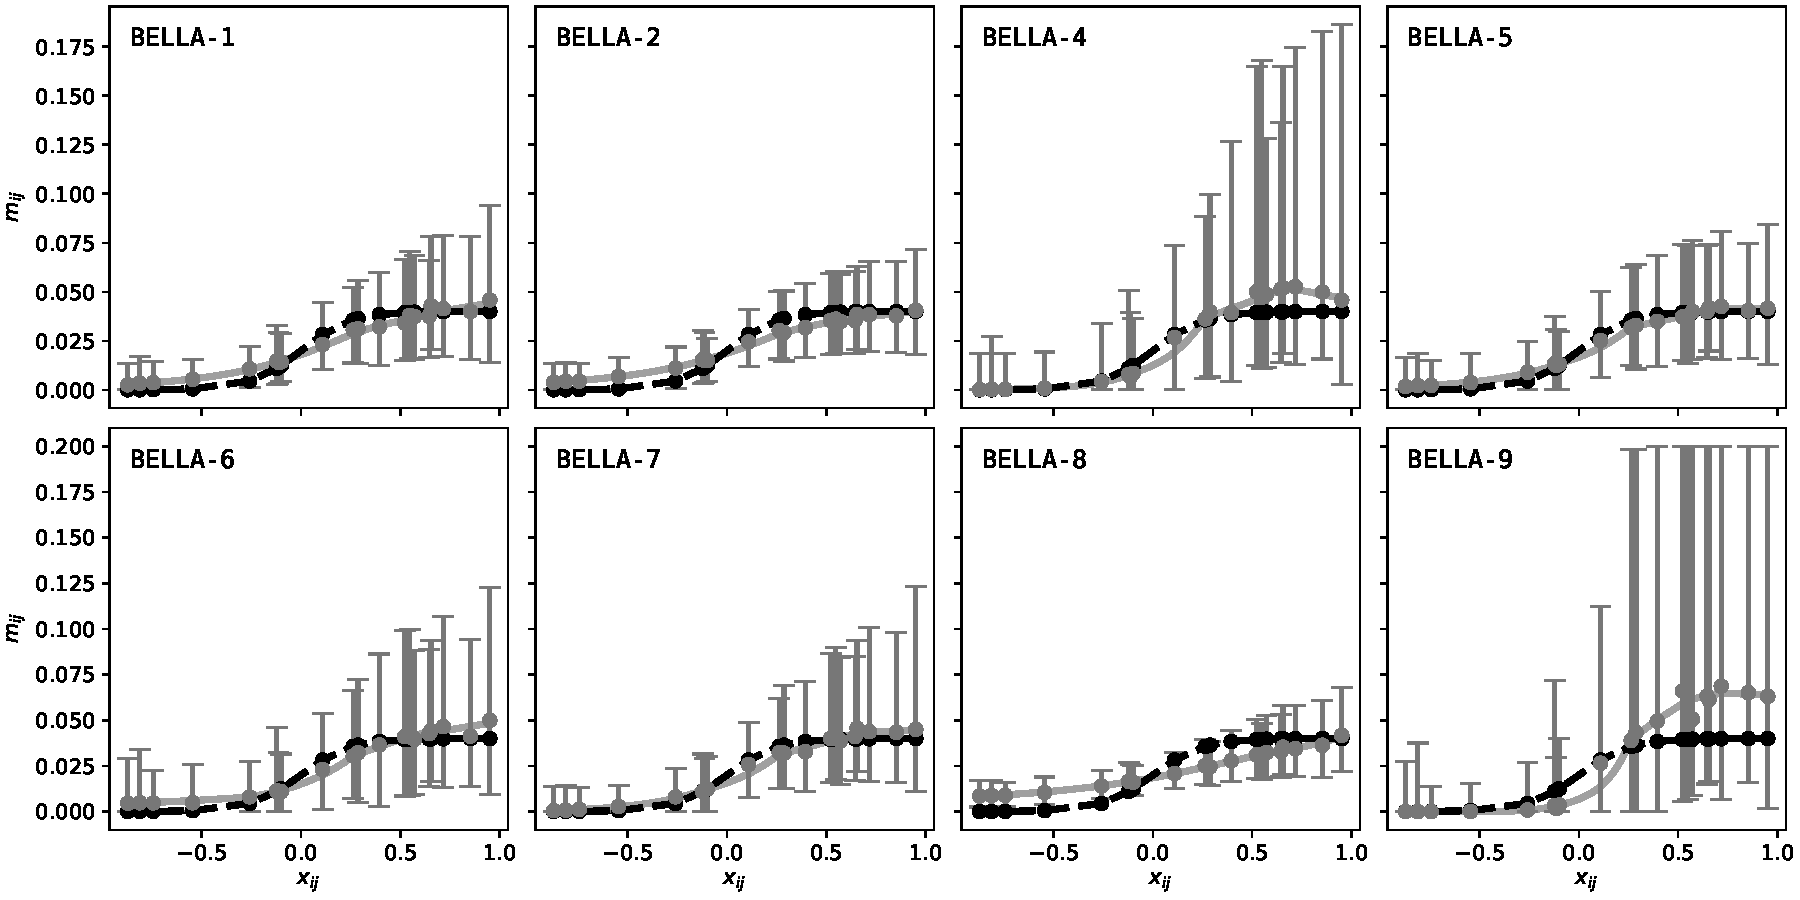
\includegraphics[width=1\textwidth]{figures/epi-multitype/sensitivity.pdf}
    \caption{Sensitivity of BELLA architecture choices for the multitype epidemiological migration-rate simulation (\texttt{Epi-4}) across 100 simulation replicates. In each panel, the points show the median posterior estimate across simulation replicates for each directed migration rate, $m_{ij}$, as a function of its migration predictor $x_{ij}$, while the vertical intervals indicate the corresponding median 95\% credible interval bounds. The colored smooth curve summarizes the fitted predictor-rate trend, and the black dashed curve with points shows the true simulated migration rates.}%
    \label{fig:epi-multitype:sensitivity}
\end{figure}

\begin{figure}[htbp]
    \centering
    
\includegraphics[width=1\textwidth]{figures/fbd-no-traits/ribbons.pdf}
    \caption{Reconstruction of birth and death rate skylines in fossilized birth-death simulations without traits across 100 simulation replicates. Rows are grouped by scenario and target: (a) \texttt{FBD-1}, (b) \texttt{FBD-2}; and (c) \texttt{FBD-2}, with the birth-rate ($\lambda$) row followed by the death-rate ($\mu$) row. Columns correspond to predictor-agnostic (PA), GLM, and BELLA-3. In each panel, the solid line shows the posterior median rate trajectory across simulation replicates, while the colored ribbons summarize its distribution, with the darker ribbon showing the 50\% interquantile range and the lighter ribbon showing the 95\% interquantile range; the black dashed line shows the true simulated rate trajectory.}%
    \label{fig:fbd-no-traits:ribbons}
\end{figure}

\begin{figure}[htbp]
    \centering
    
\includegraphics[width=1\textwidth]{figures/fbd-no-traits/metrics.pdf}
    \caption{Time-resolved diagnostics for fossilized birth-death simulations without traits across 100 simulation replicates. Rows are grouped by scenario and target: (a) \texttt{FBD-1}, (b) \texttt{FBD-2}; and (c) \texttt{FBD-2}, with the birth-rate ($\lambda$) row followed by the death-rate ($\mu$). Columns show mean absolute percentage error (MAPE), empirical coverage, and coefficient of variation by time bin. Colored distributions or lines compare predictor-agnostic (PA), GLM, and \texttt{BELLA-3}; MAPE and coefficient of variation are evaluated per replicate, whereas coverage is evaluated as the fraction of intervals containing the true rate value in each time bin.}%
    \label{fig:fbd-no-traits:metrics}
\end{figure}

\begin{figure}[htbp]
    \centering
    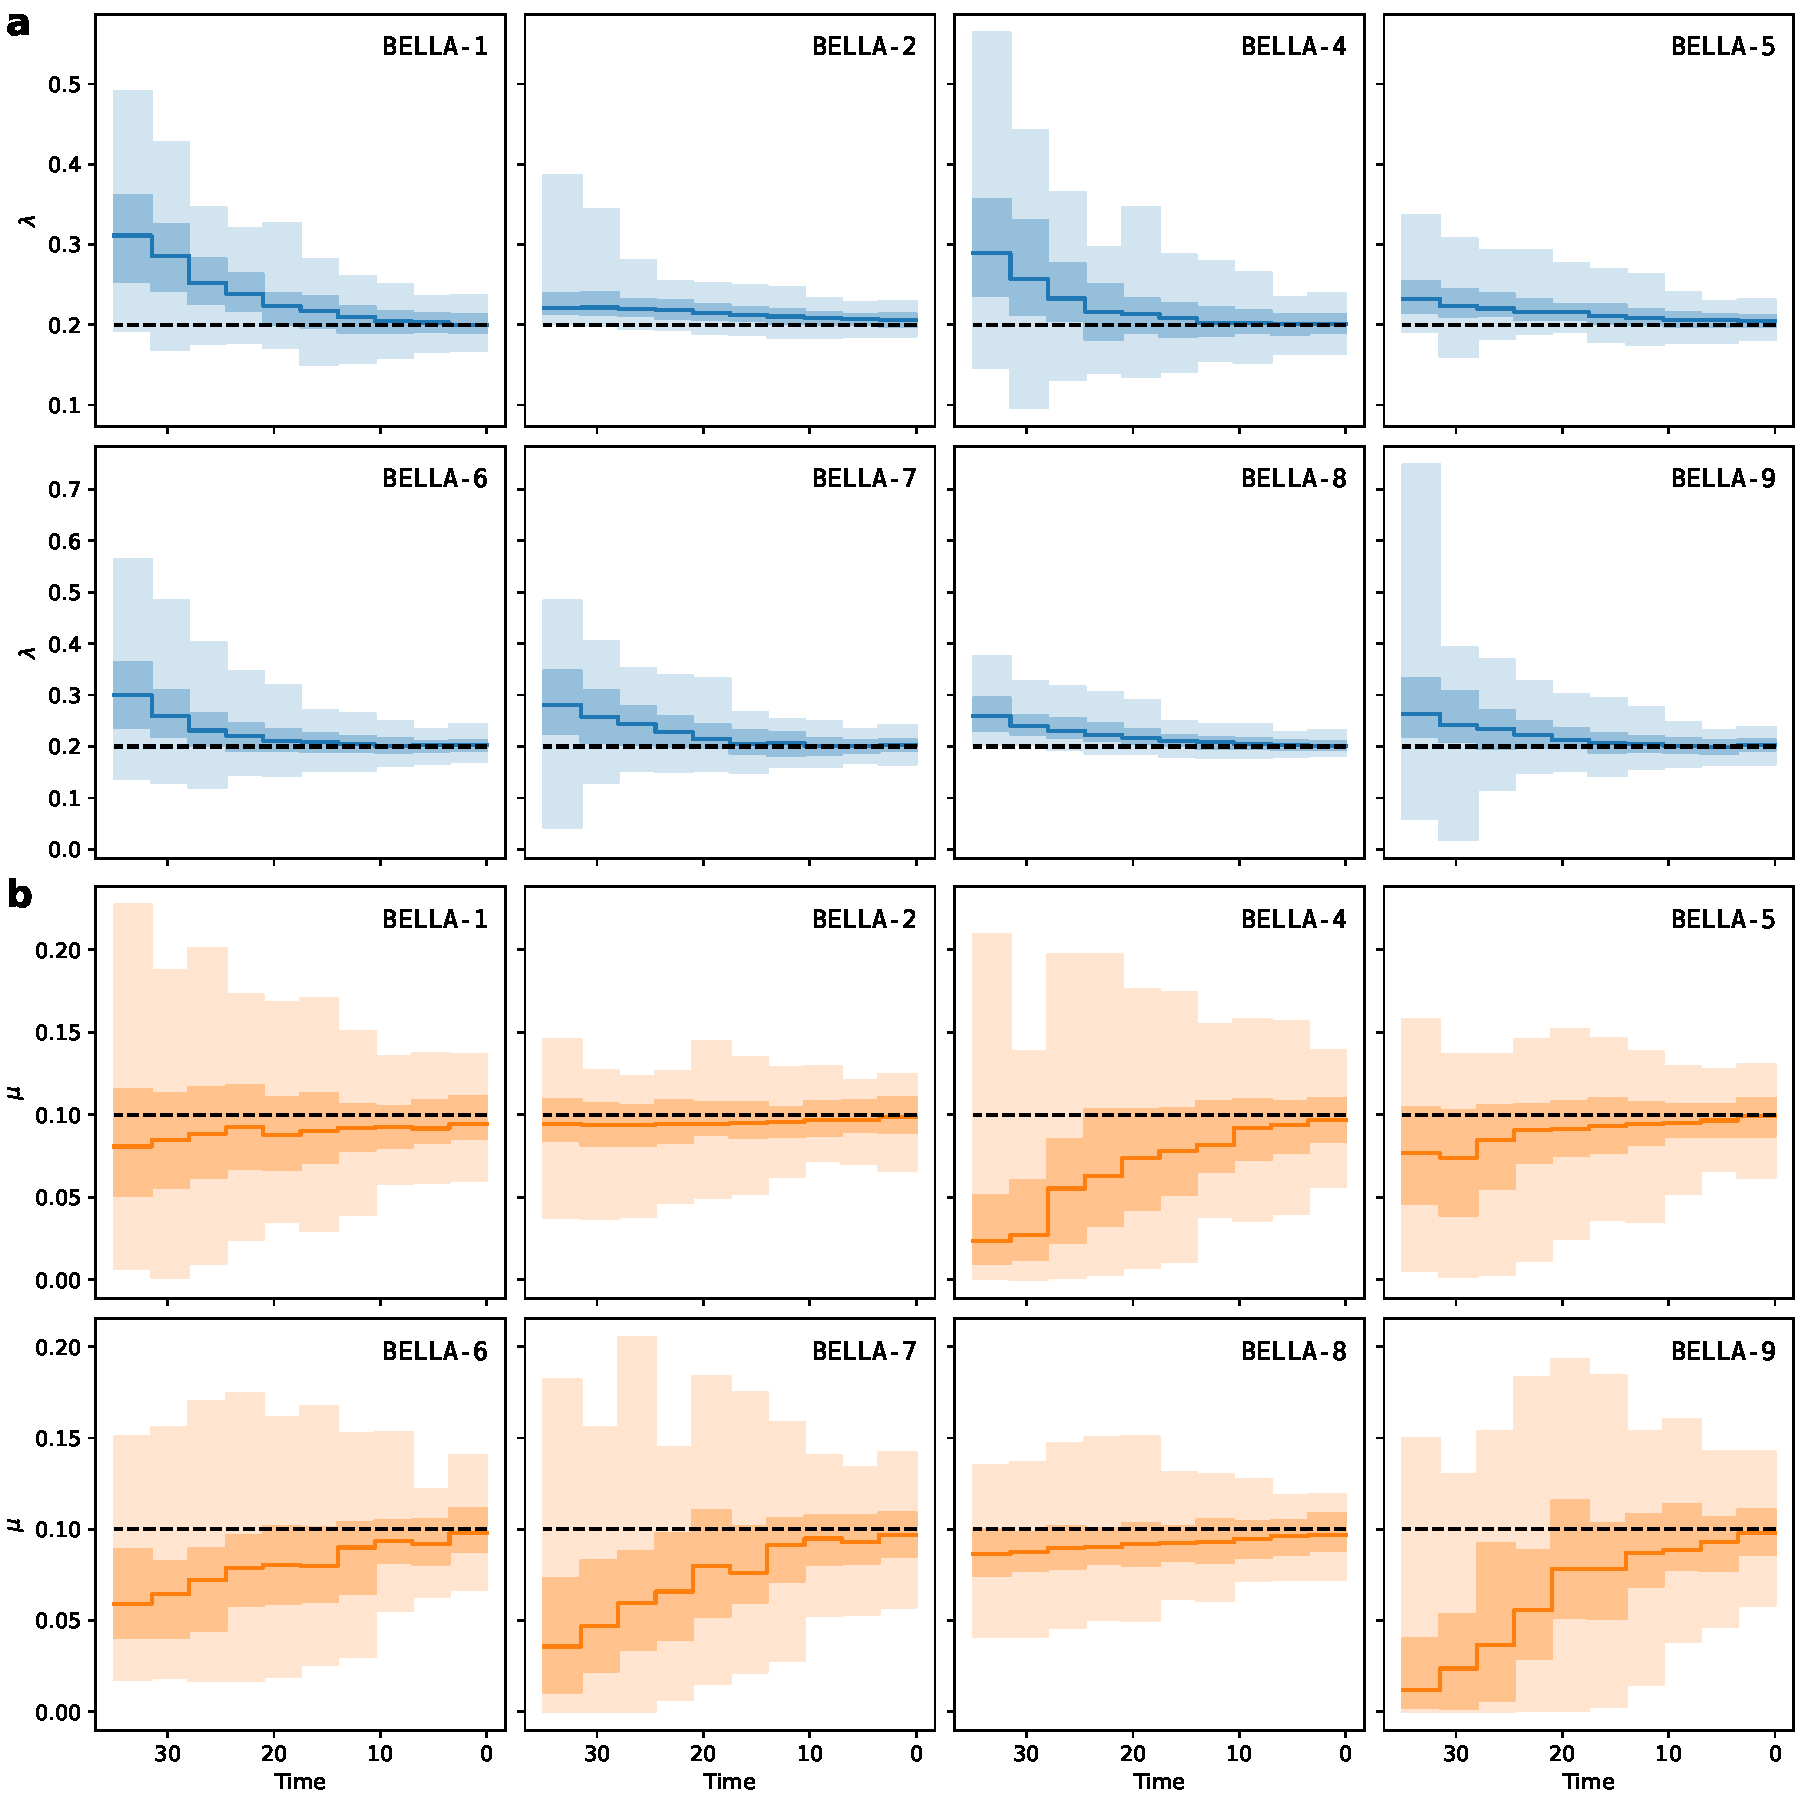
\includegraphics[width=1\textwidth]{figures/fbd-no-traits/sensitivity/fbd-no-traits_1.pdf}
    \caption{Sensitivity of BELLA architecture choices for \texttt{FBD-1} across 100 simulation replicates. (a) Birth-rate ($\lambda$) estimates, shown in the first two rows. (b) Death-rate ($\mu$) estimates, shown in the last two rows. In each panel, the solid line shows the posterior median rate trajectory across simulation replicates, while the colored ribbons summarize its distribution, with the darker ribbon showing the 50\% interquantile range and the lighter ribbon showing the 95\% interquantile range; the black dashed line shows the true simulated rate trajectory.}%
    \label{fig:fbd-no-traits:sensitivity:fbd-no-traits_1}
\end{figure}

\begin{figure}[htbp]
    \centering
    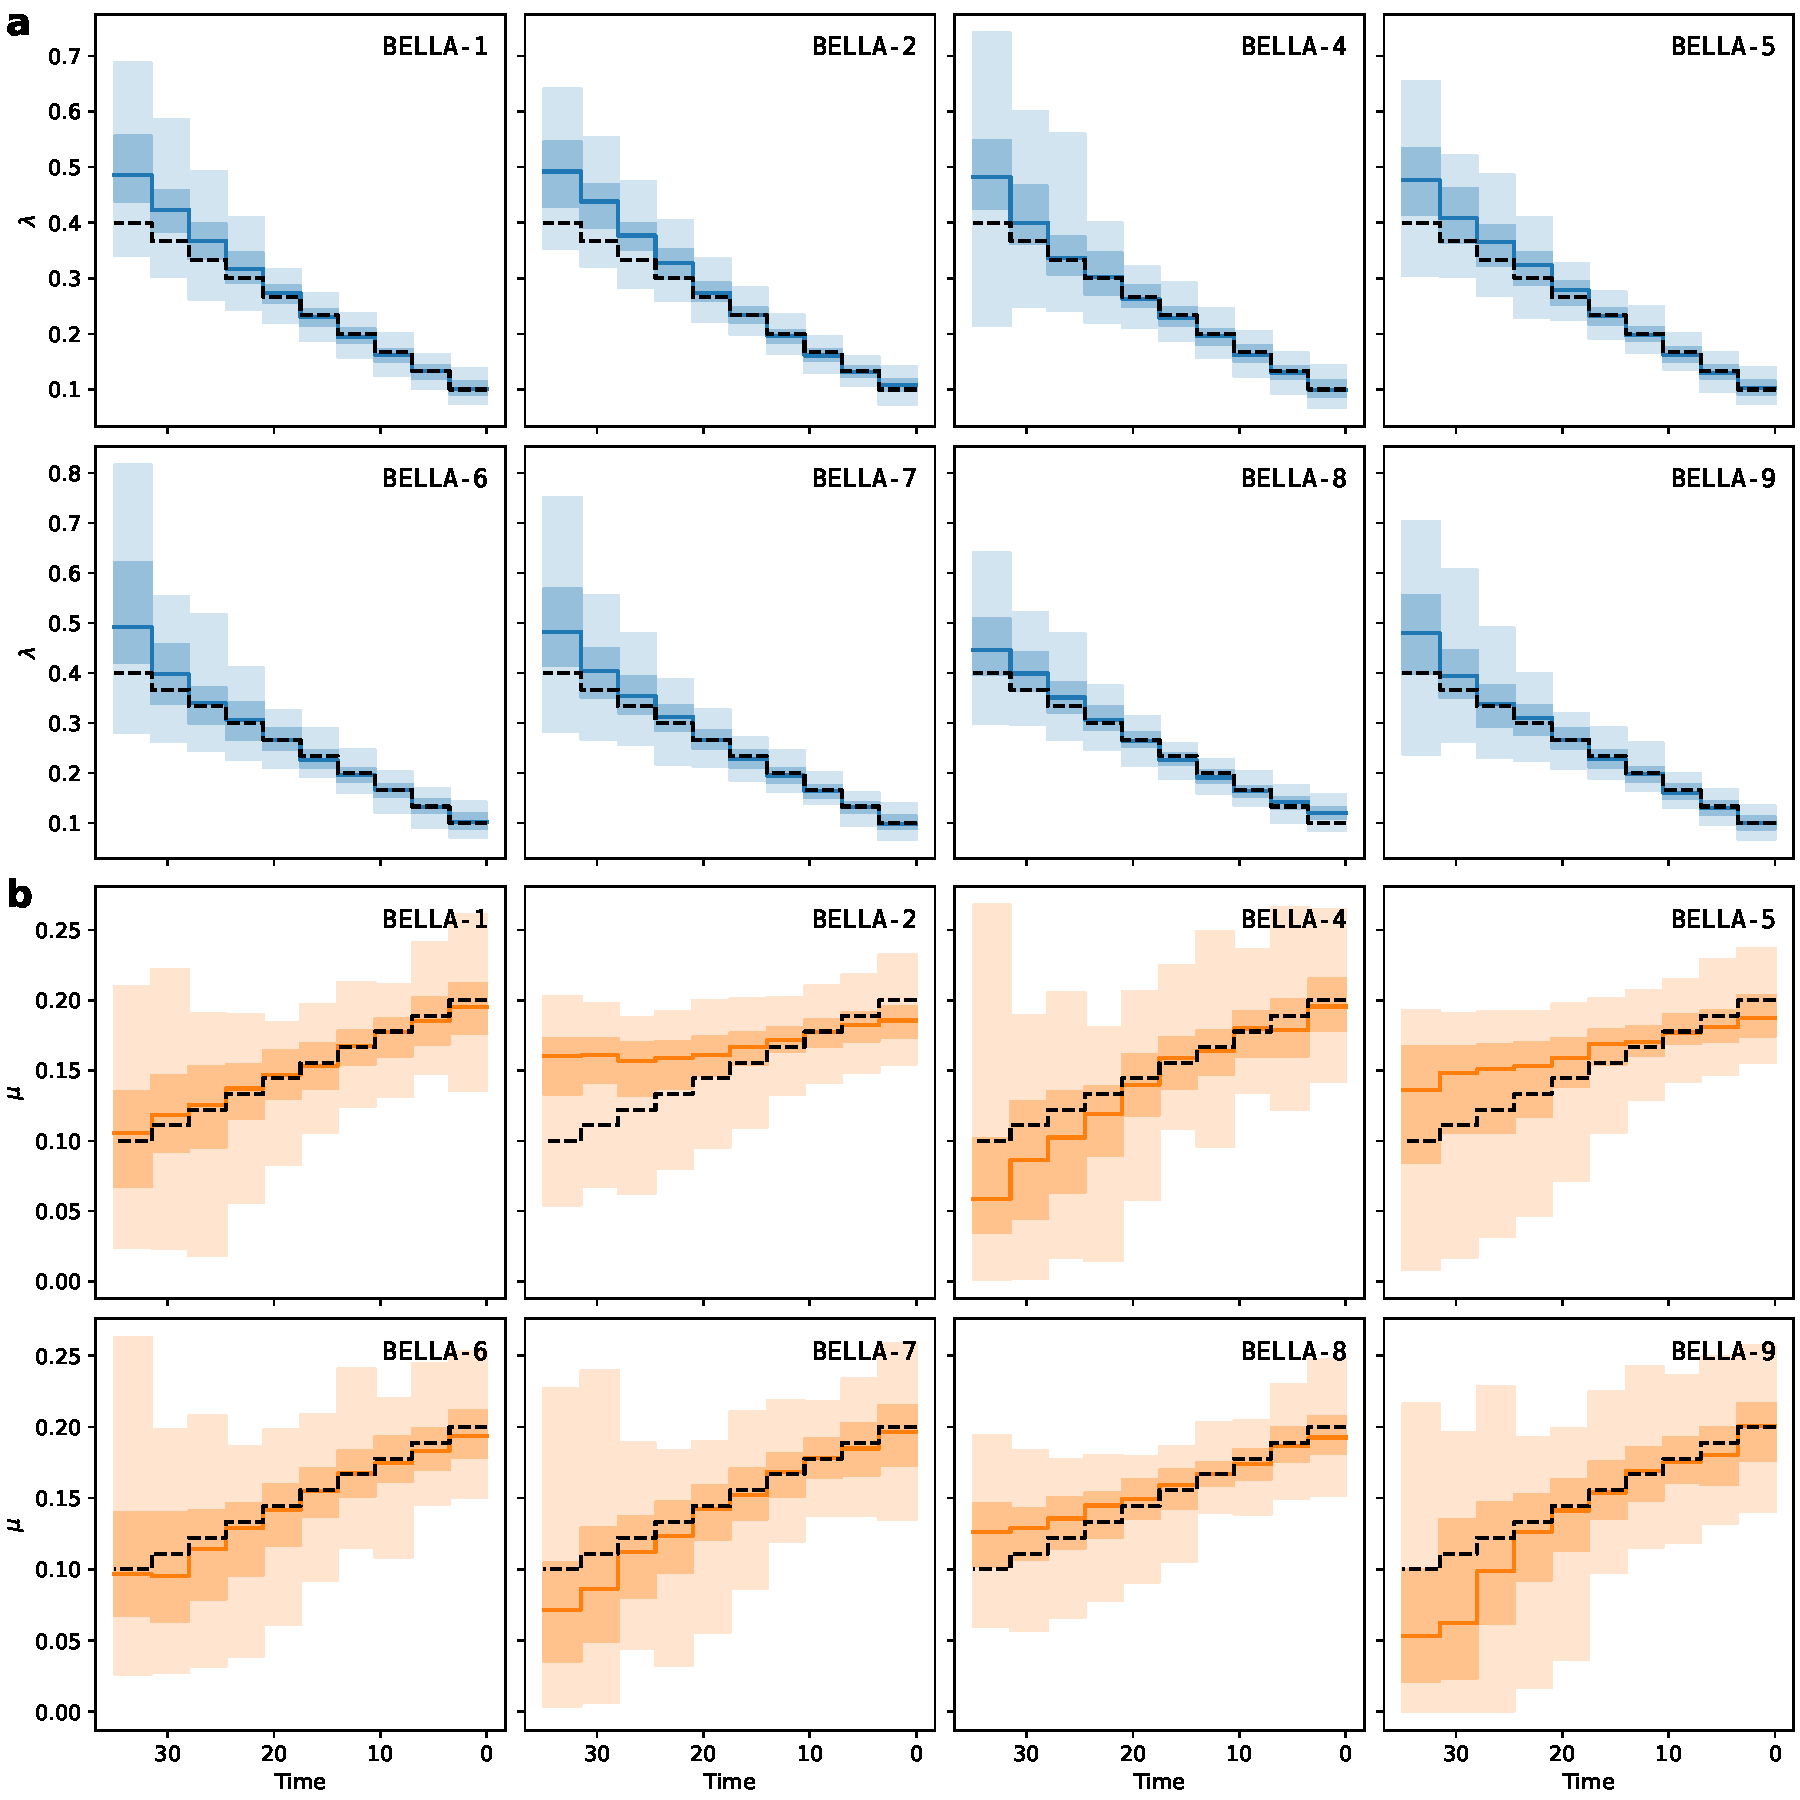
\includegraphics[width=1\textwidth]{figures/fbd-no-traits/sensitivity/fbd-no-traits_2.pdf}
    \caption{Sensitivity of BELLA architecture choices for \texttt{FBD-2} across 100 simulation replicates. (a) Birth-rate ($\lambda$) estimates, shown in the first two rows. (b) Death-rate ($\mu$) estimates, shown in the last two rows. In each panel, the solid line shows the posterior median rate trajectory across simulation replicates, while the colored ribbons summarize its distribution, with the darker ribbon showing the 50\% interquantile range and the lighter ribbon showing the 95\% interquantile range; the black dashed line shows the true simulated rate trajectory.}%
    \label{fig:fbd-no-traits:sensitivity:fbd-no-traits_2}
\end{figure}

\begin{figure}[htbp]
    \centering
    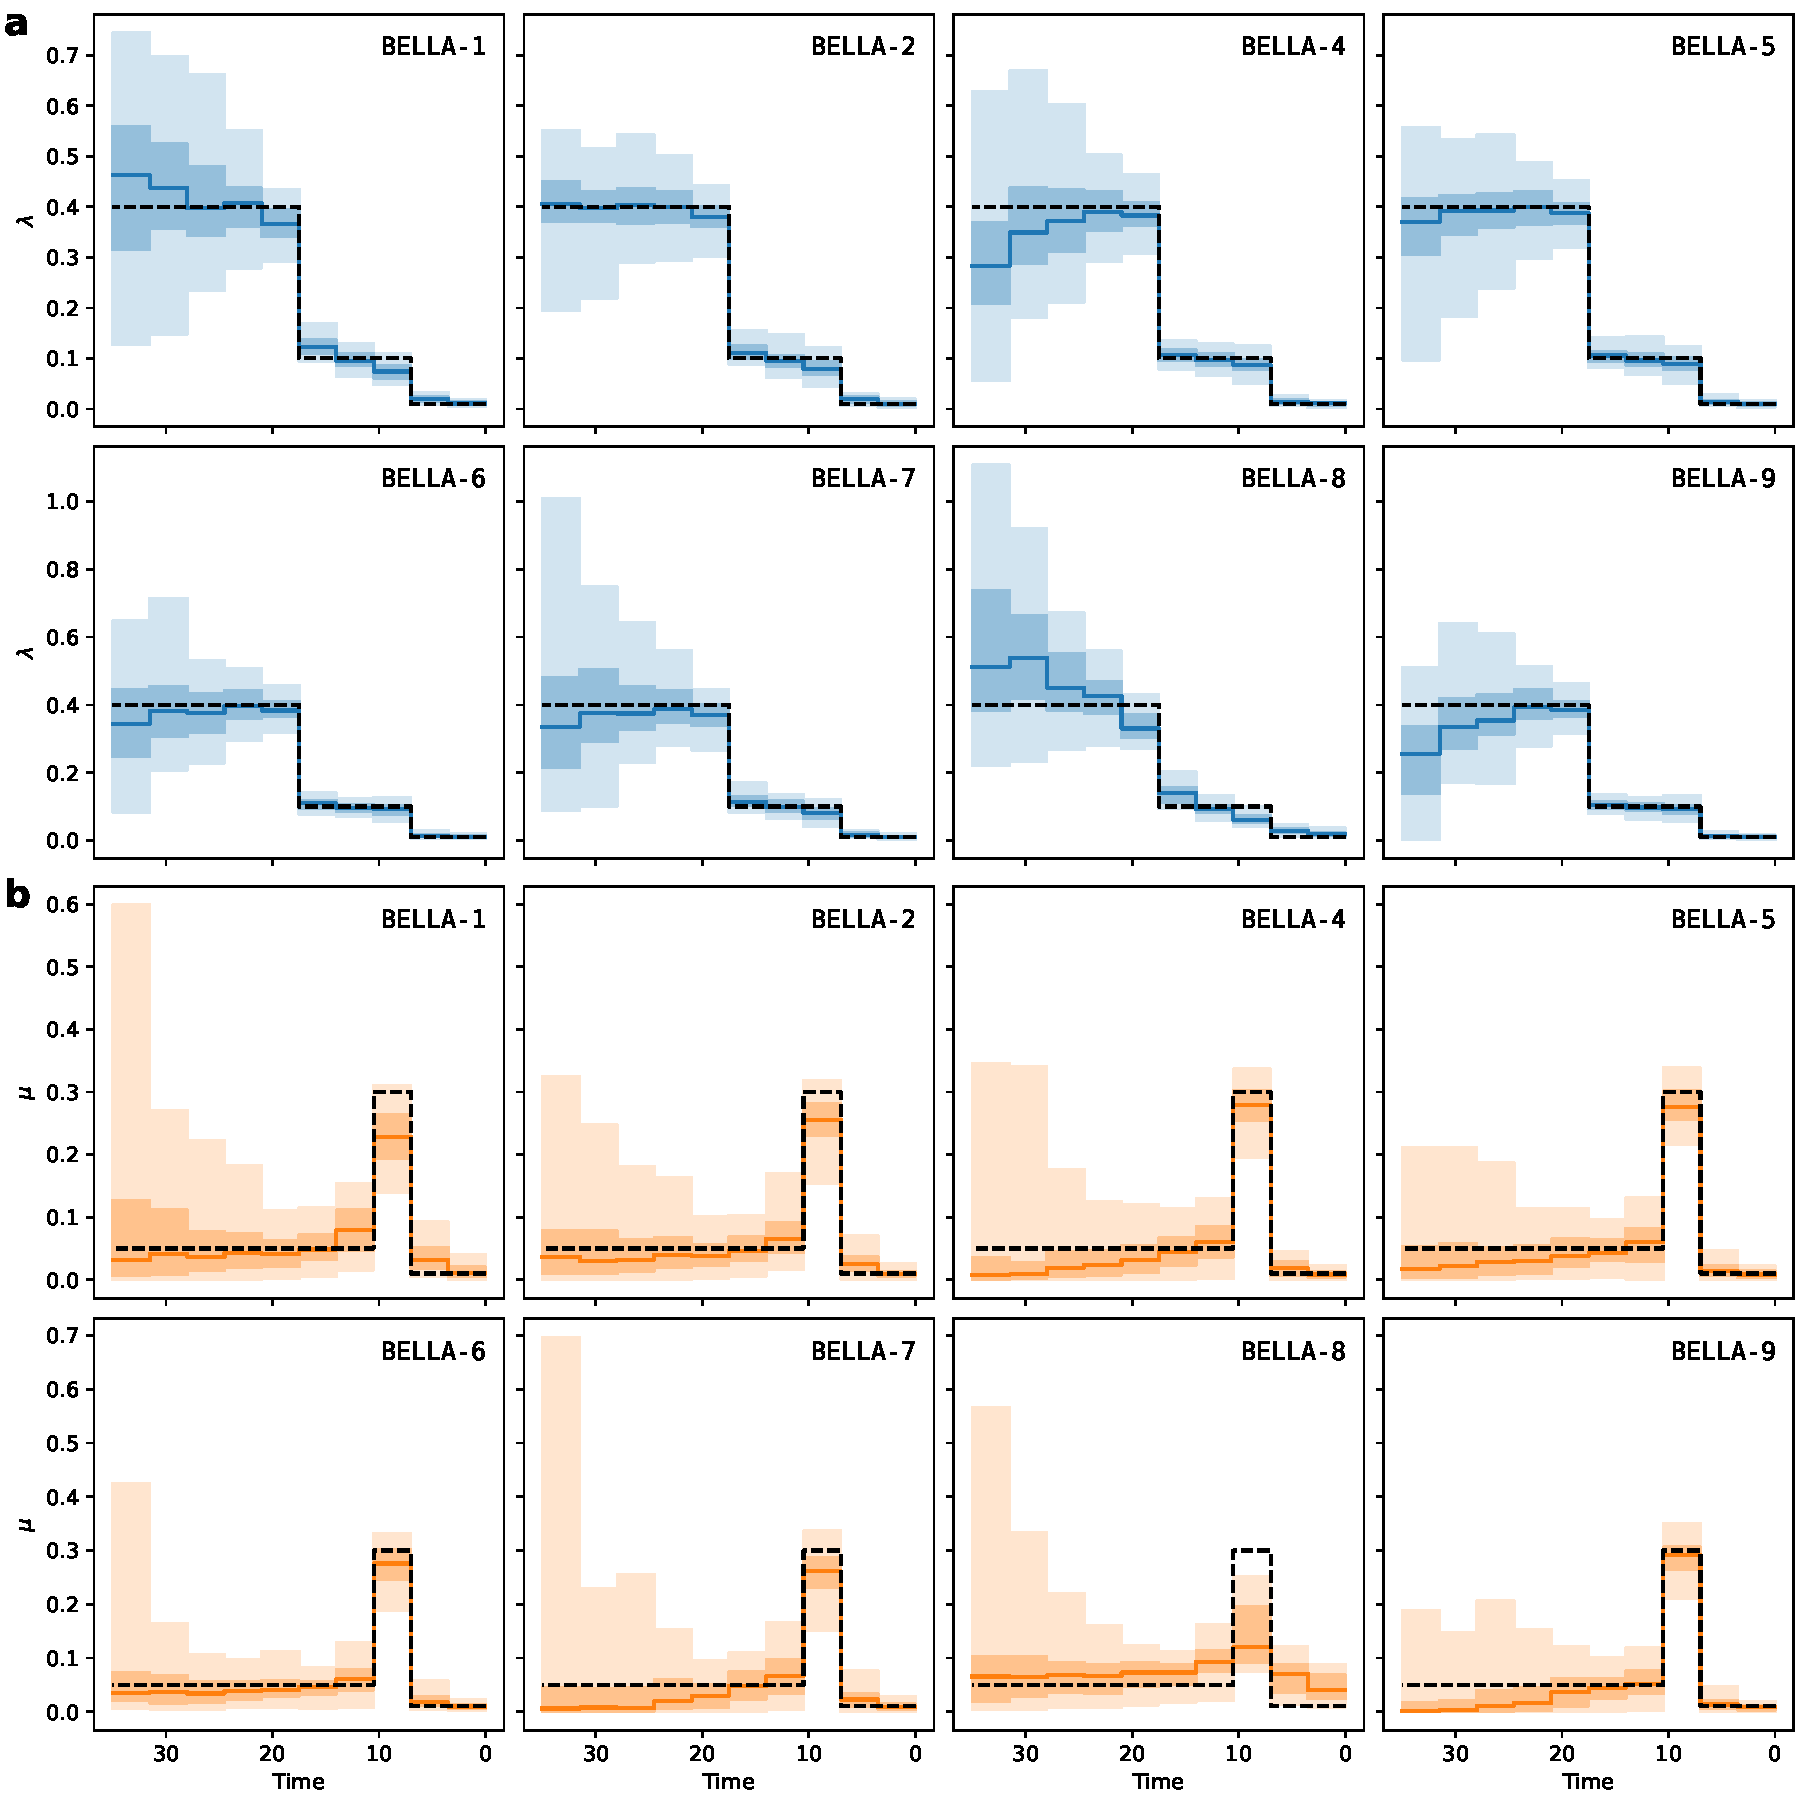
\includegraphics[width=1\textwidth]{figures/fbd-no-traits/sensitivity/fbd-no-traits_3.pdf}
    \caption{Sensitivity of BELLA architecture choices for \texttt{FBD-3} across 100 simulation replicates. (a) Birth-rate ($\lambda$) estimates, shown in the first two rows. (b) Death-rate ($\mu$) estimates, shown in the last two rows. In each panel, the solid line shows the posterior median rate trajectory across simulation replicates, while the colored ribbons summarize its distribution, with the darker ribbon showing the 50\% interquantile range and the lighter ribbon showing the 95\% interquantile range; the black dashed line shows the true simulated rate trajectory.}%
    \label{fig:fbd-no-traits:sensitivity:fbd-no-traits_3}
\end{figure}

\begin{figure}[htbp]
    \centering
    
\includegraphics[width=0.8\textwidth]{figures/fbd-2traits/metrics.pdf}
    \caption{Time-resolved diagnostics for the fossilized birth--death simulation with two binary traits (\texttt{FBD-4}) across 100 simulation replicates. Rows are grouped by target rate: (a) speciation-rate diagnostics, $\lambda^{(s)}$, for the four binary trait states $s \in {00, 01, 10, 11}$, shown in consecutive rows, followed by (b) extinction-rate diagnostics, $\mu^{(s)}$, for the same states. Columns show mean absolute percentage error (MAPE), empirical coverage, and coefficient of variation by time bin. Colored distributions or lines compare predictor-agnostic (PA), GLM, and \texttt{BELLA-4}; MAPE and coefficient of variation are evaluated per replicate, whereas coverage is evaluated as the fraction of intervals containing the true rate value in each time bin.}%
    \label{fig:fbd-2traits:metrics}
\end{figure}

\begin{figure}[htbp]
    \centering
    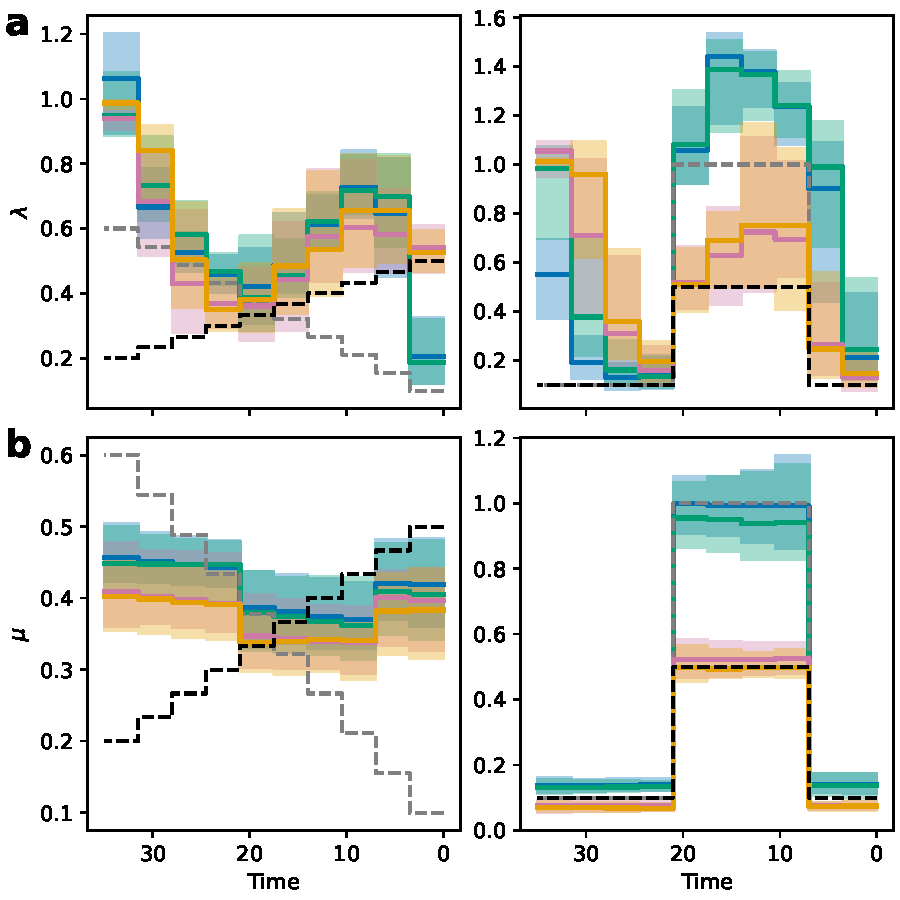
\includegraphics[width=1\textwidth]{figures/fbd-2traits/benchmark.pdf}
    \caption{(a) Predictor-agnostic (PA) and (b) GLM estimates of the state-specific speciation and extinction rate skylines, $\lambda$ and $\mu$, for the fossilized birth--death simulation with two binary traits (\texttt{FBD-4}) across 100 simulation replicates. In each panel, the solid colored lines represent the median trajectories across simulation replicates for the four binary trait states: $00$ (blue), $01$ (green), $10$ (pink), and $11$ (orange), while the colored ribbons represent the corresponding 50\% interquantile ranges. Dashed lines indicate the true simulated rates, shown in black when the first trait is in state $1$ and in gray when it is in state $0$.}%
    \label{fig:fbd-2traits:benchmark}
\end{figure}

\begin{figure}[htbp]
    \centering
    
\includegraphics[width=1\textwidth]{figures/fbd-2traits/sensitivity.pdf}
    \caption{Sensitivity of BELLA architecture choices for the fossilized birth--death simulation with two binary traits (\texttt{FBD-4}) across 100 simulation replicates. (a) Birth-rate ($\lambda$) estimates, shown in the first two rows. (b) Death-rate ($\mu$) estimates, shown in the last two rows. In each panel, the solid colored lines represent the median trajectories across simulation replicates for the four binary trait states: $00$ (blue), $01$ (green), $10$ (pink), and $11$ (orange), while the colored ribbons represent the corresponding 50\% interquantile ranges. Dashed lines indicate the true simulated rates, shown in black when the first trait is in state $1$ and in gray when it is in state $0$.}%
    \label{fig:fbd-2traits:sensitivity}
\end{figure}

\begin{figure}[htpb]
    
\includegraphics[width=1\textwidth]{figures/platyrrhine/ribbons.pdf}
    \caption{Results of BELLA for the diversification analysis of 100 New World monkey (Platyrrhines) phylogenies. Columns (left to right) show the speciation rate \( \lambda \), the extinction rate \( \mu \), and the diversification rate \( d = \lambda - \mu \). The four rows correspond to the four body-mass categories (from smallest to largest), and display the median posterior rate (solid line) and its distribution, summarized by the 50\% and 95\% percentile intervals (dark and light shaded ribbons, respectively).}%
    \label{fig:platyrrhine:ribbons}
\end{figure}

\begin{figure}[htpb]
    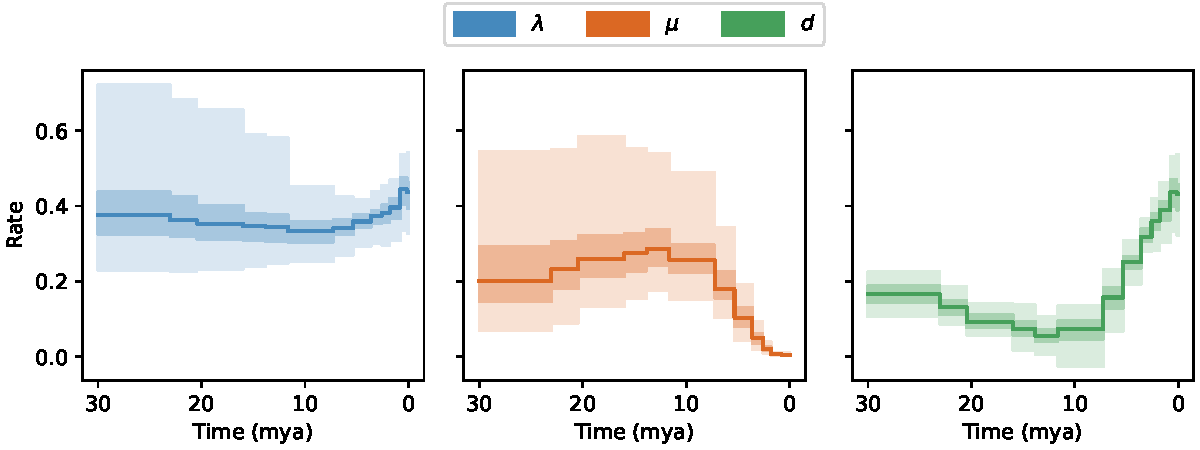
\includegraphics[width=1\textwidth]{figures/platyrrhine/marginal.pdf}
    \caption{Results of BELLA for the diversification analysis of 100 New World monkey (Platyrrhines) phylogenies. Columns (left to right) show the marginal speciation rate \( \lambda \), the marginal extinction rate \( \mu \), and the marginal diversification rate \( d = \lambda - \mu \). For each time bin, rates were averaged across body-mass classes, weighted by the number of lineages in each class. Solid lines represent the median posterior rates across phylogenies, while shaded ribbons summarize their distribution, with darker and lighter bands denoting the 50\% and 95\% percentile intervals, respectively.}%
    \label{fig:platyrrhine:marginal}
\end{figure}

\begin{figure}[htpb]
    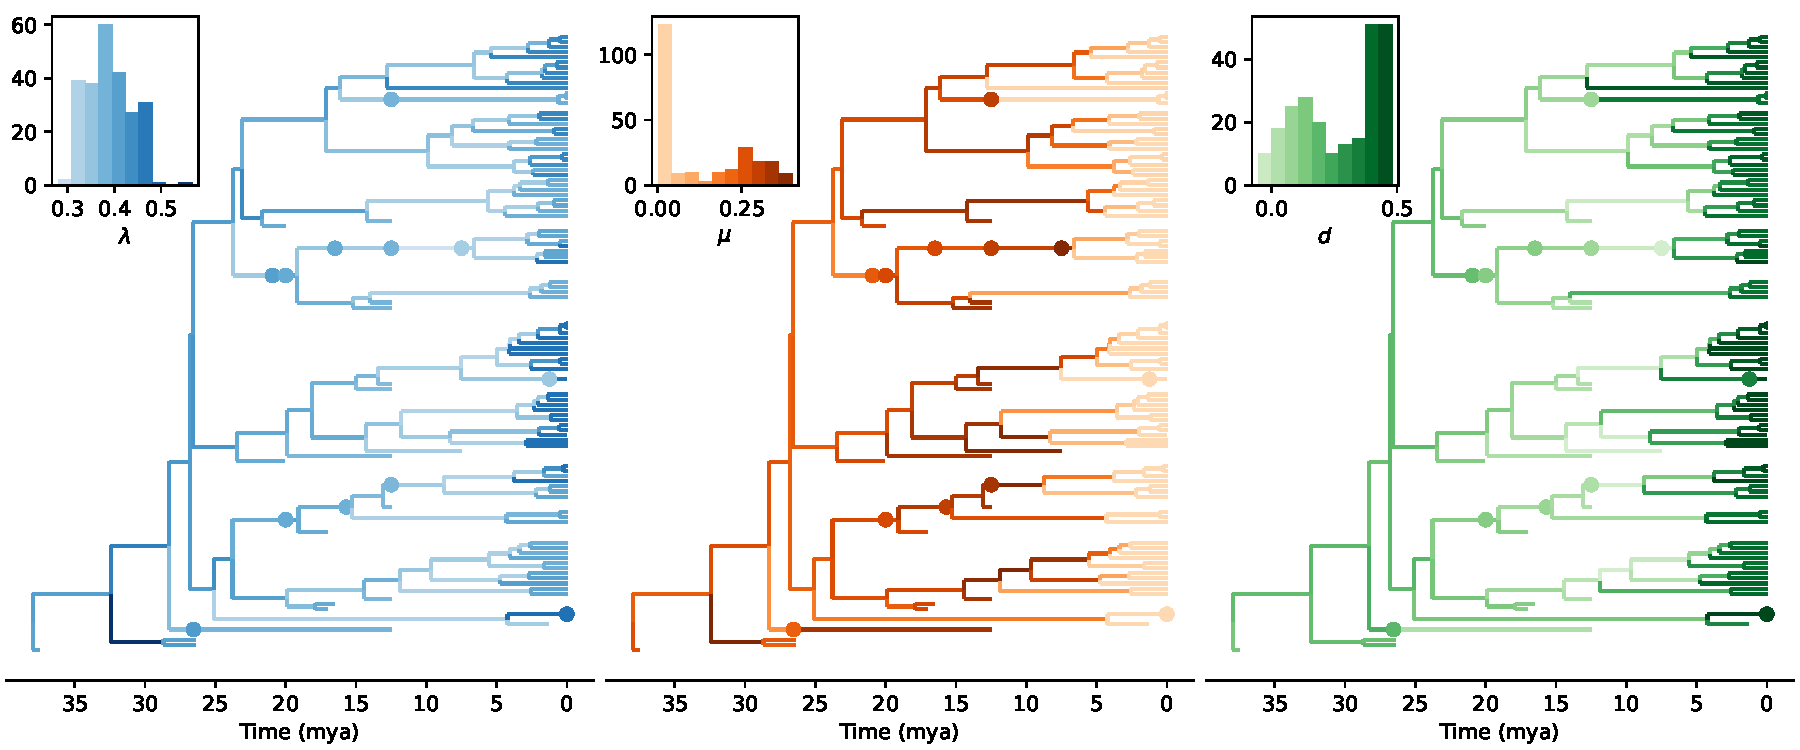
\includegraphics[width=1\textwidth]{figures/platyrrhine/trees.pdf}
    \caption{Results of BELLA for the diversification analysis of 100 New World monkeys (Platyrrhines) phylogenies. From left to right, the panels show: the speciation rate (\( \lambda \), blue), the extinction rate (\( \mu \), orange) and (c) the diversification rate (\( d = \lambda - \mu \), green) mapped onto the maximum clade credibility tree. Each panel includes an inset histogram illustrating the distribution of the corresponding rate across the tree.}%
    \label{fig:platyrrhine:trees}
\end{figure}

\begin{figure}[htpb]
    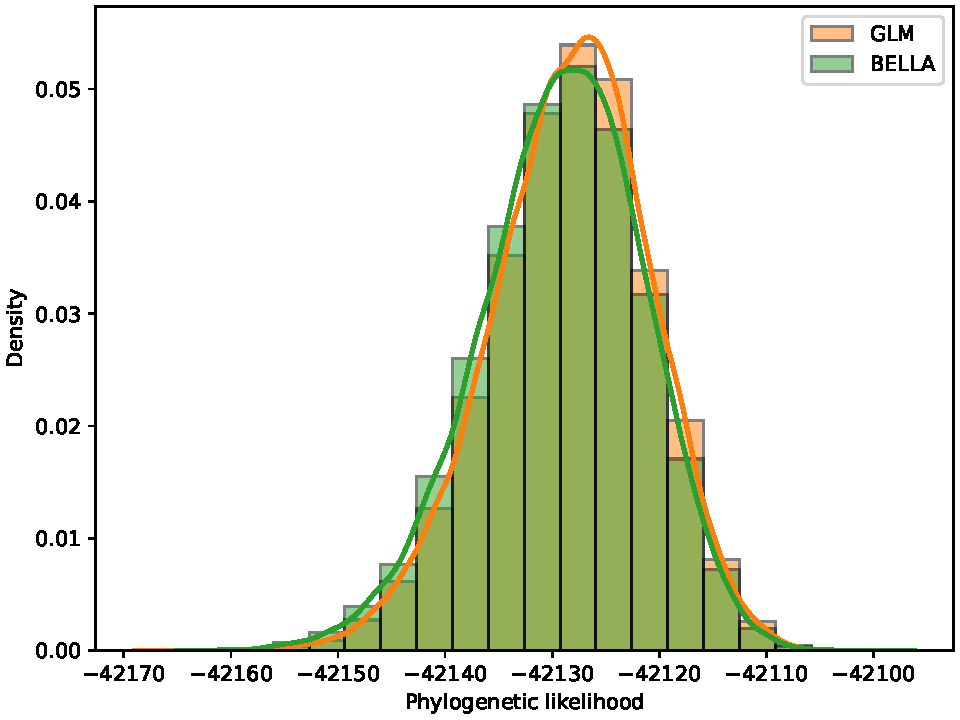
\includegraphics[width=1\textwidth]{figures/eucovid/likelihood.pdf}
    \caption{Phylogenetic likelihood distributions for the early spread of SARS-CoV-2 in Europe.}%
    \label{fig:eucovid:likelihood}
\end{figure}

\begin{figure}[htbp]
    \centering
    
\includegraphics[angle=90, width=0.8\textwidth]{figures/eucovid/cophylo.pdf}
    \caption{Cophylogeny comparing maximum clade credibility (MCC) trees from BELLA and GLM analyses for the early spread of SARS-CoV-2 in Europe. Lines connect identical taxa between trees.}
    \label{fig:eucovid:cophylo}
\end{figure}

\begin{figure}[htpb]
    
\includegraphics[width=0.6\textwidth]{figures/eucovid/GLM-tree.pdf}
    \caption{Inferred transmission tree for the early spread of SARS-CoV-2 in Europe using a GLM model.}
    \label{fig:eucovid:GLM-tree}
\end{figure}

\begin{figure}[htpb]
    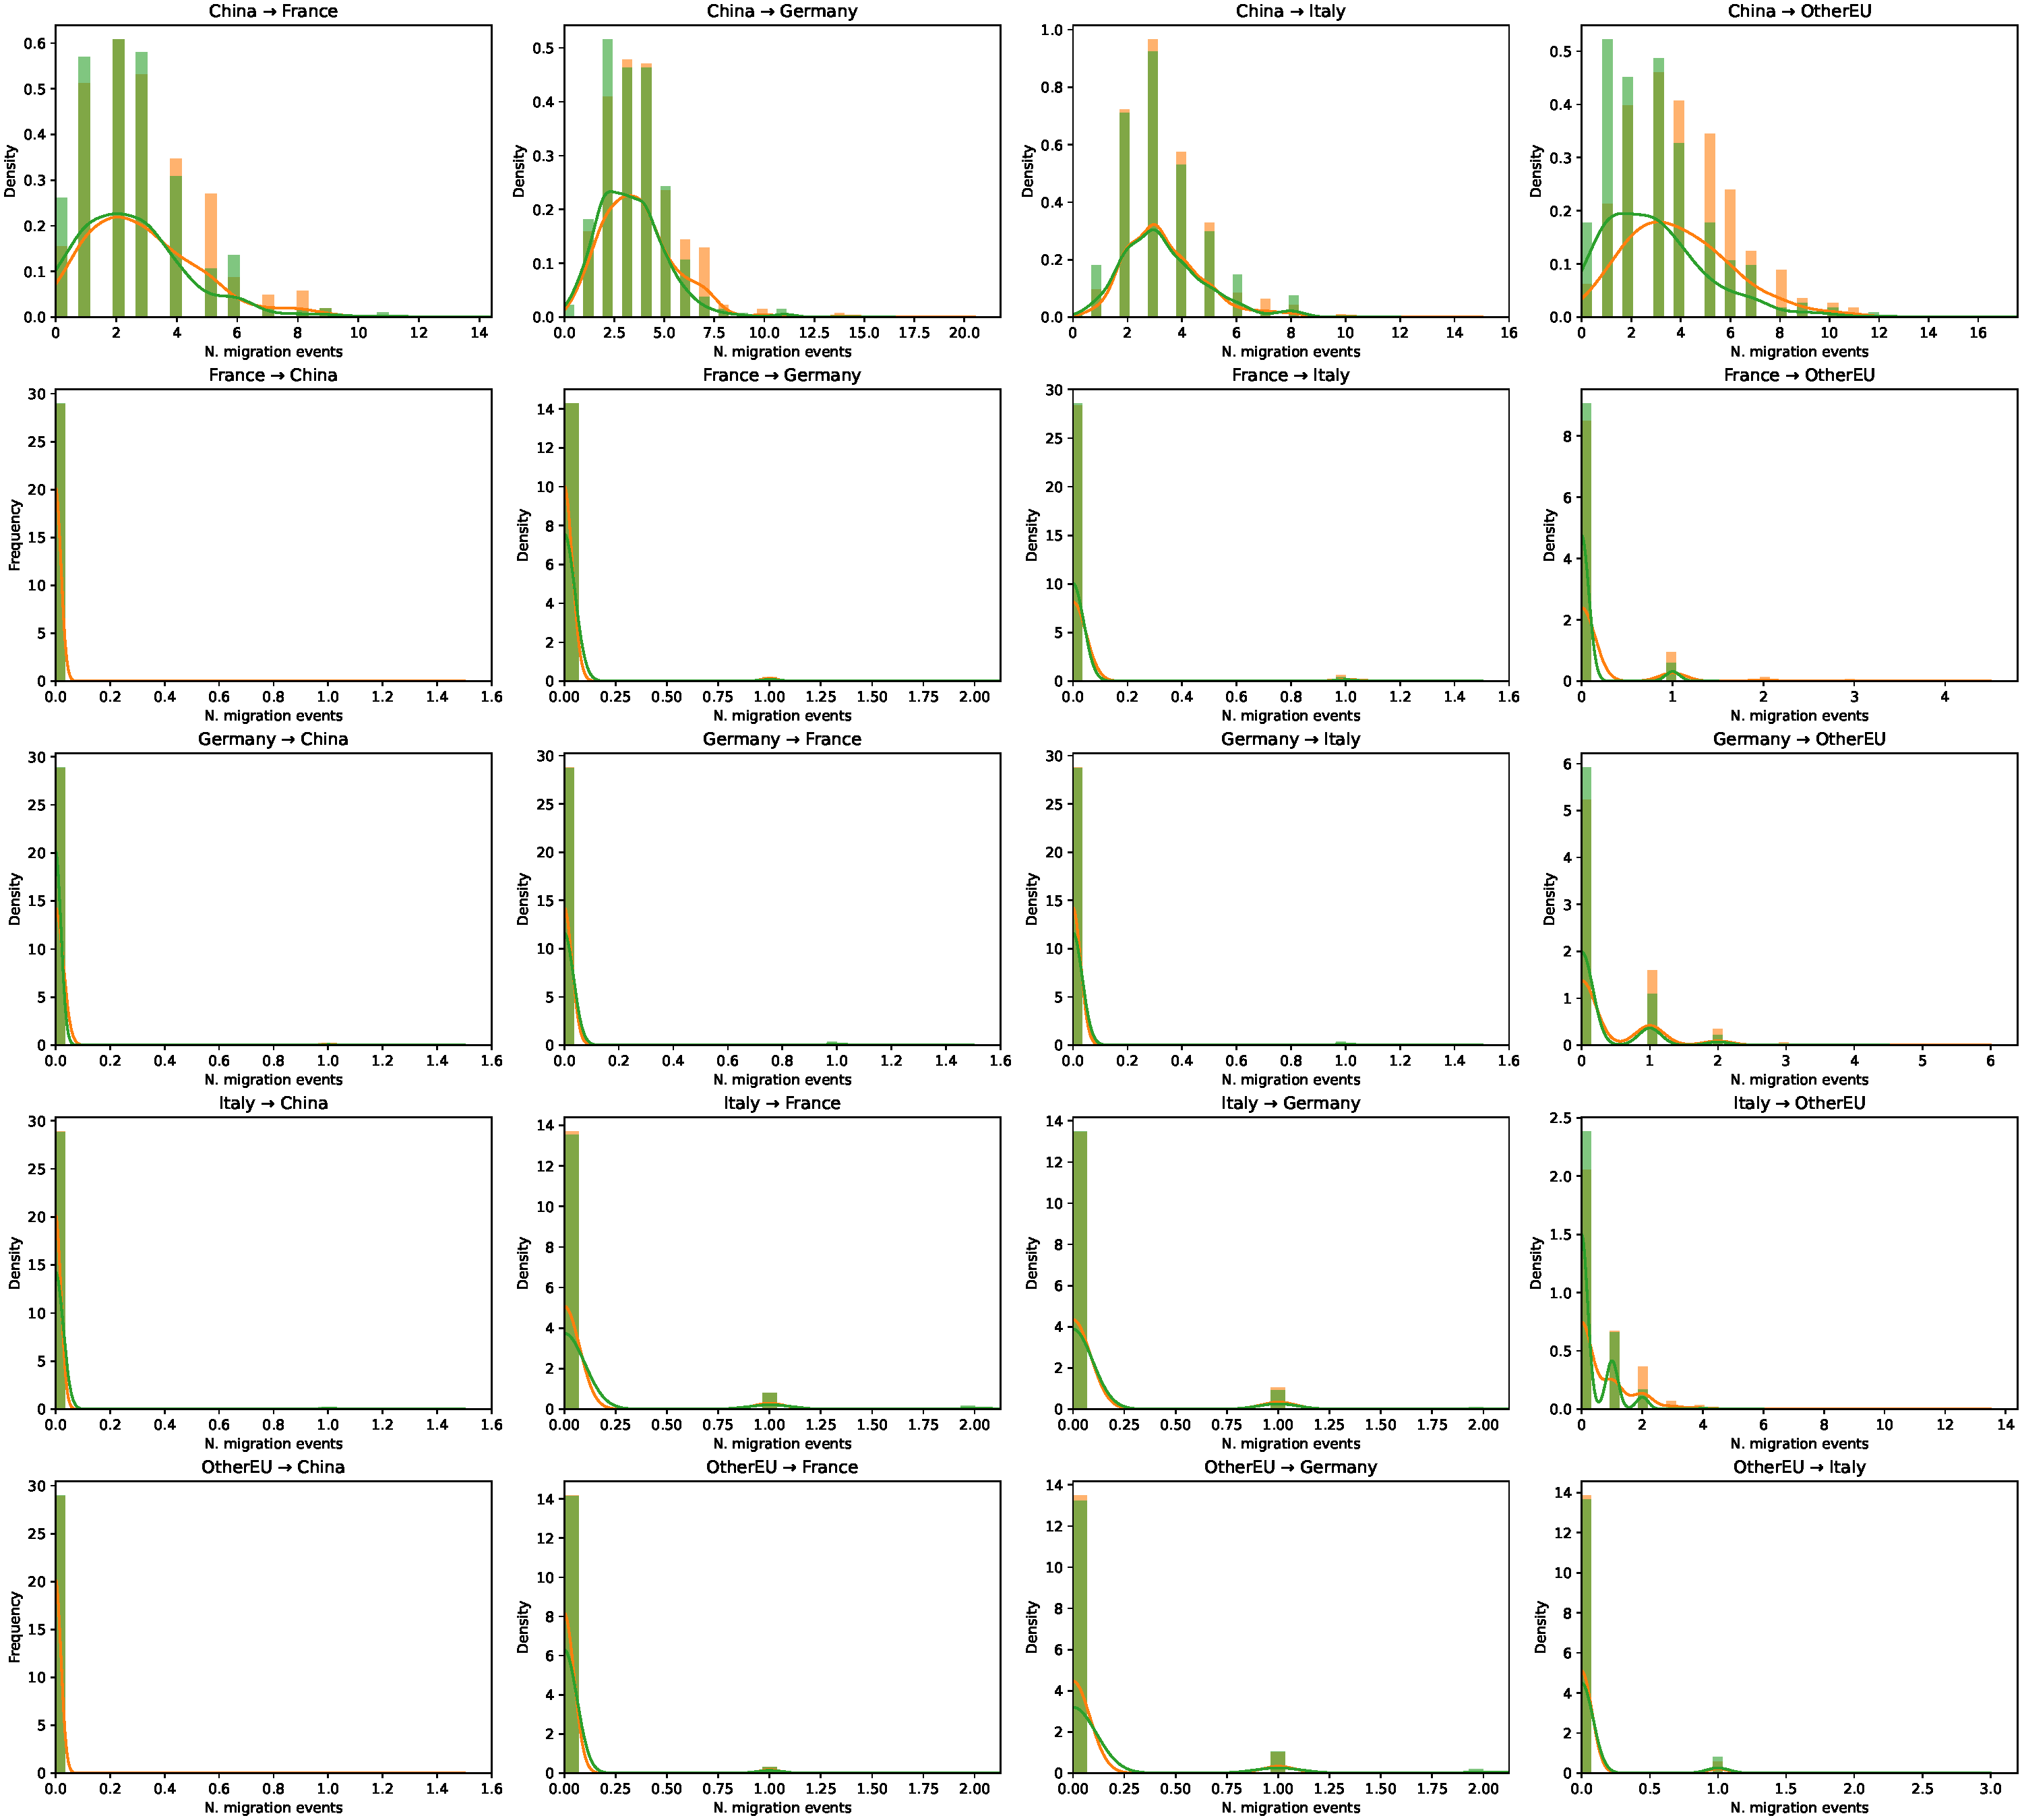
\includegraphics[width=1\textwidth]{figures/eucovid/migrations/time_bin_0.pdf}
    \caption{Distribution of estimated migration fluxes between countries during the early spread of SARS-CoV-2 in Europe for the period from 5 January 2020 to 26 January 2020.}
    \label{fig:eucovid:migrations:time_bin_0}
\end{figure}

\begin{figure}[htpb]
    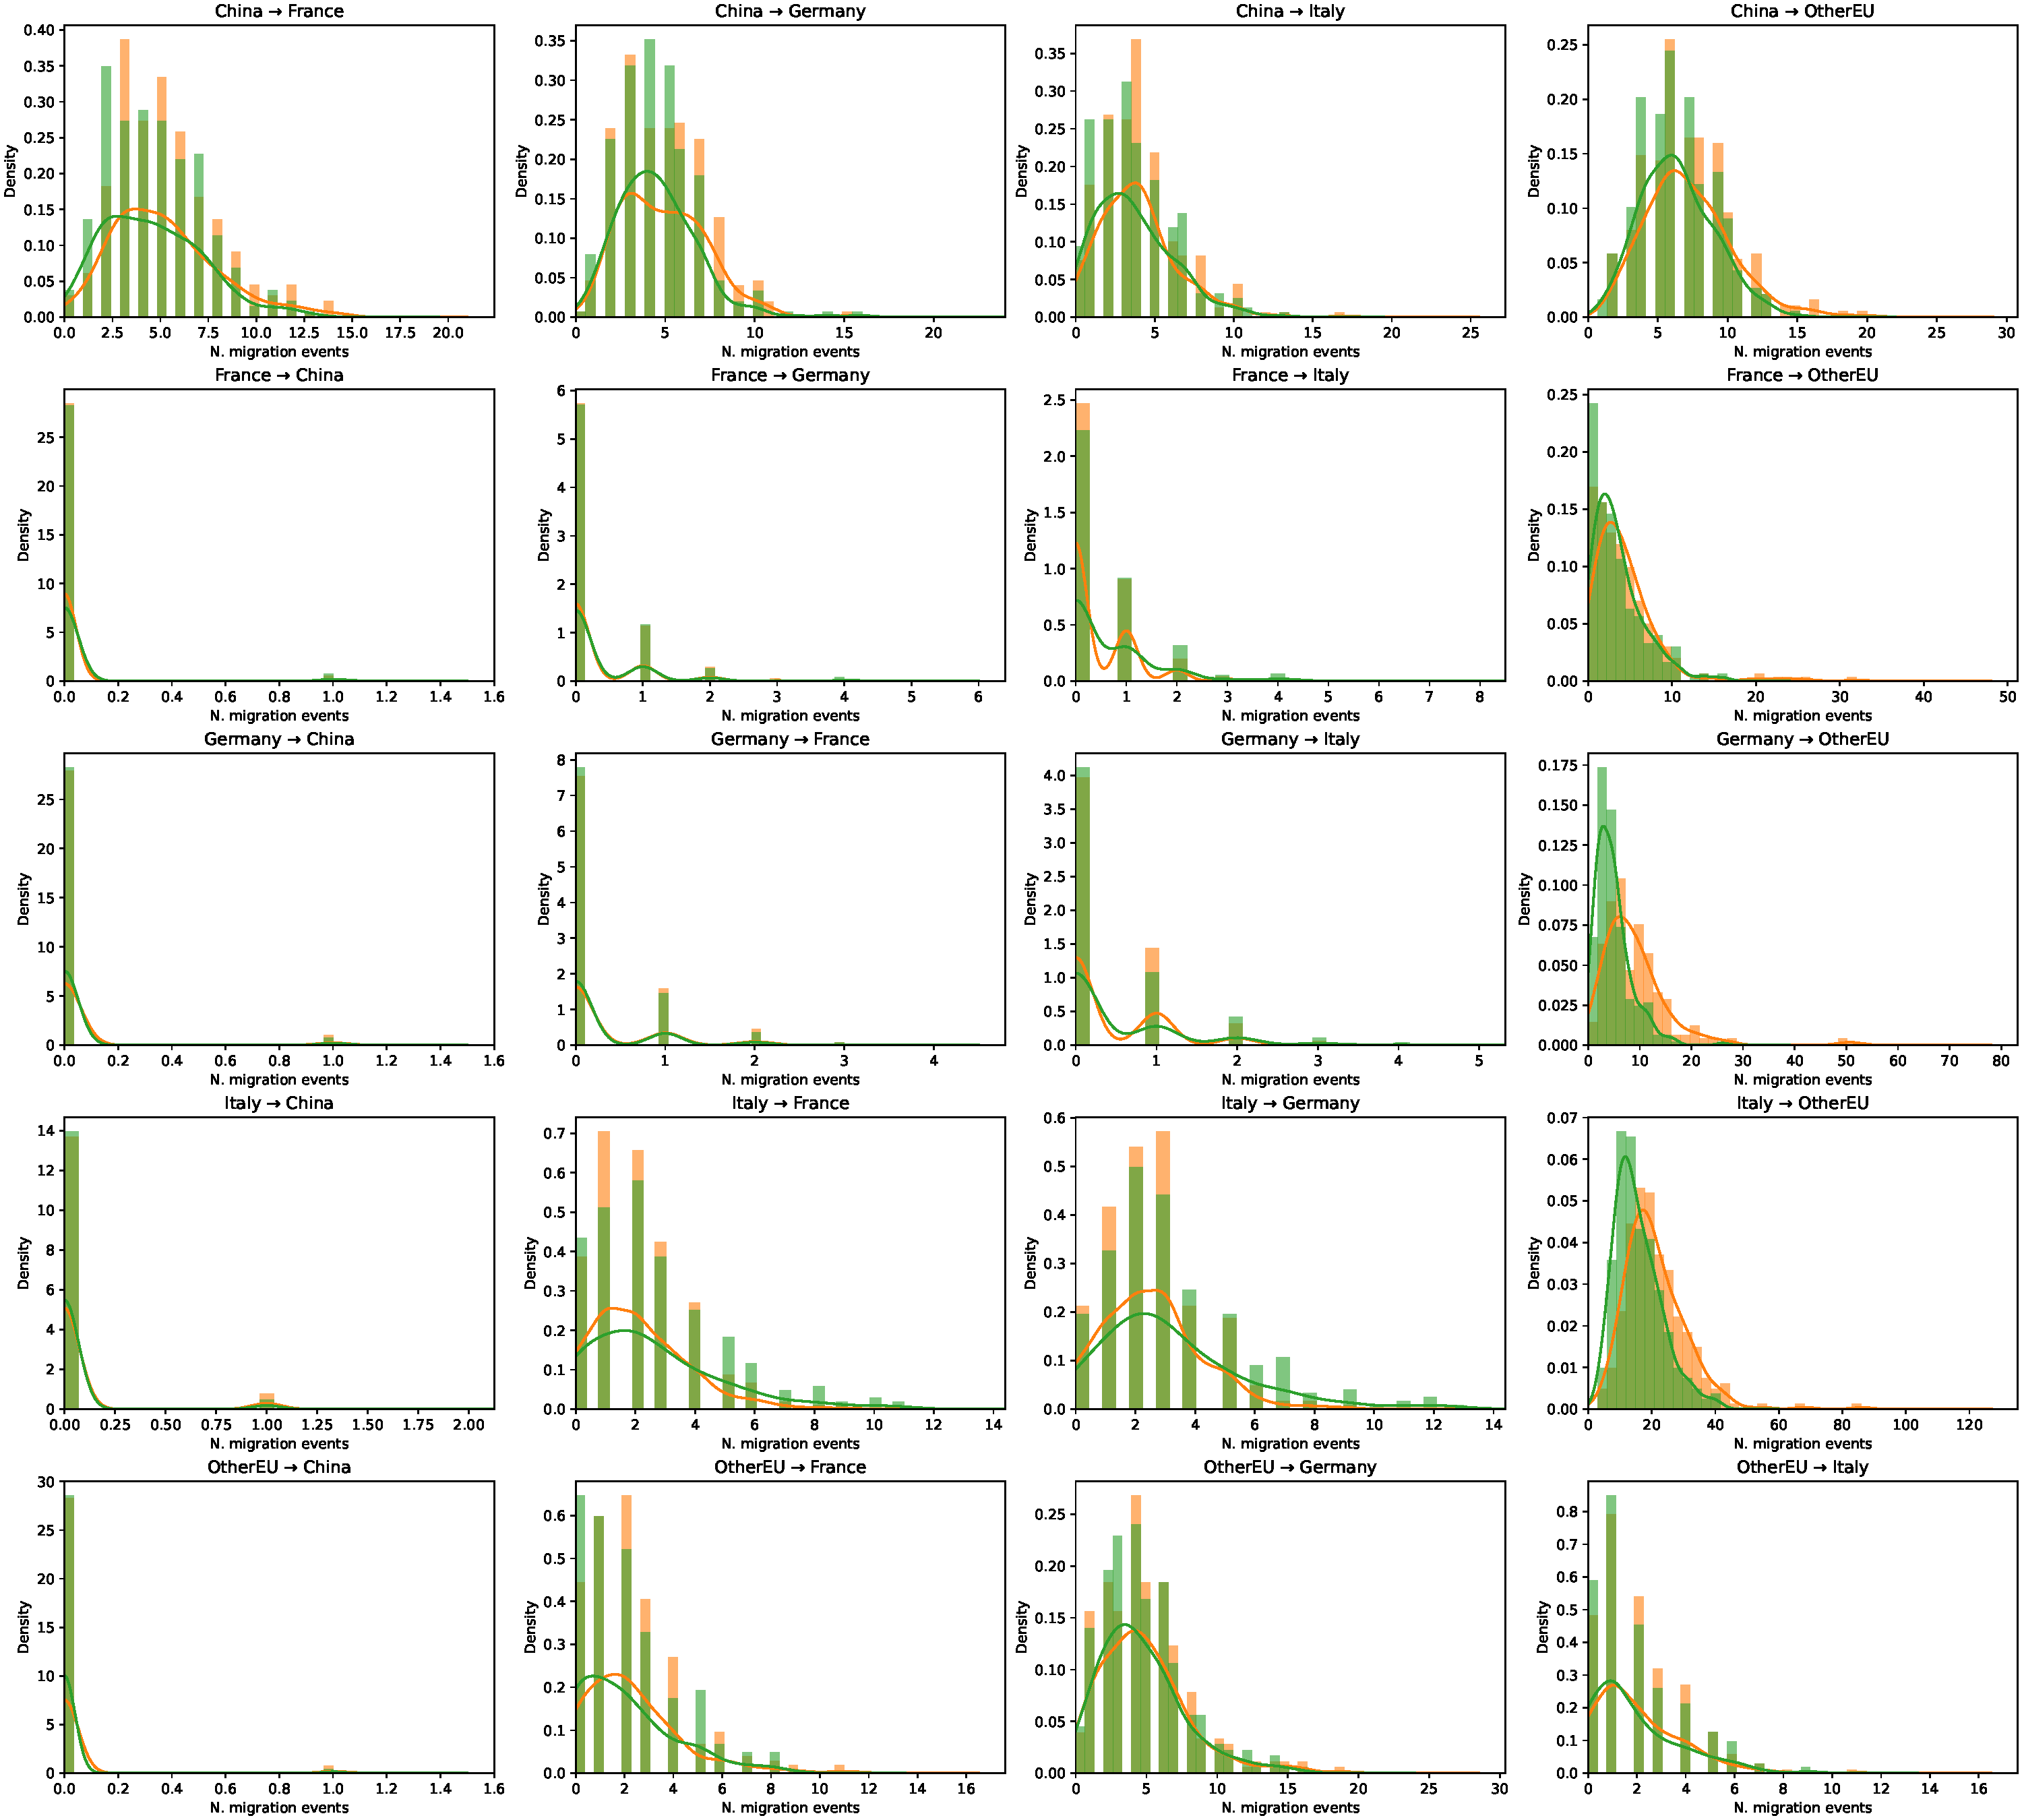
\includegraphics[width=1\textwidth]{figures/eucovid/migrations/time_bin_1.pdf}
    \caption{Distribution of estimated migration fluxes between countries during the early spread of SARS-CoV-2 in Europe for the period from 26 January 2020 to 16 February 2020.}
    \label{fig:eucovid:migrations:time_bin_1}
\end{figure}

\begin{figure}[htpb]
    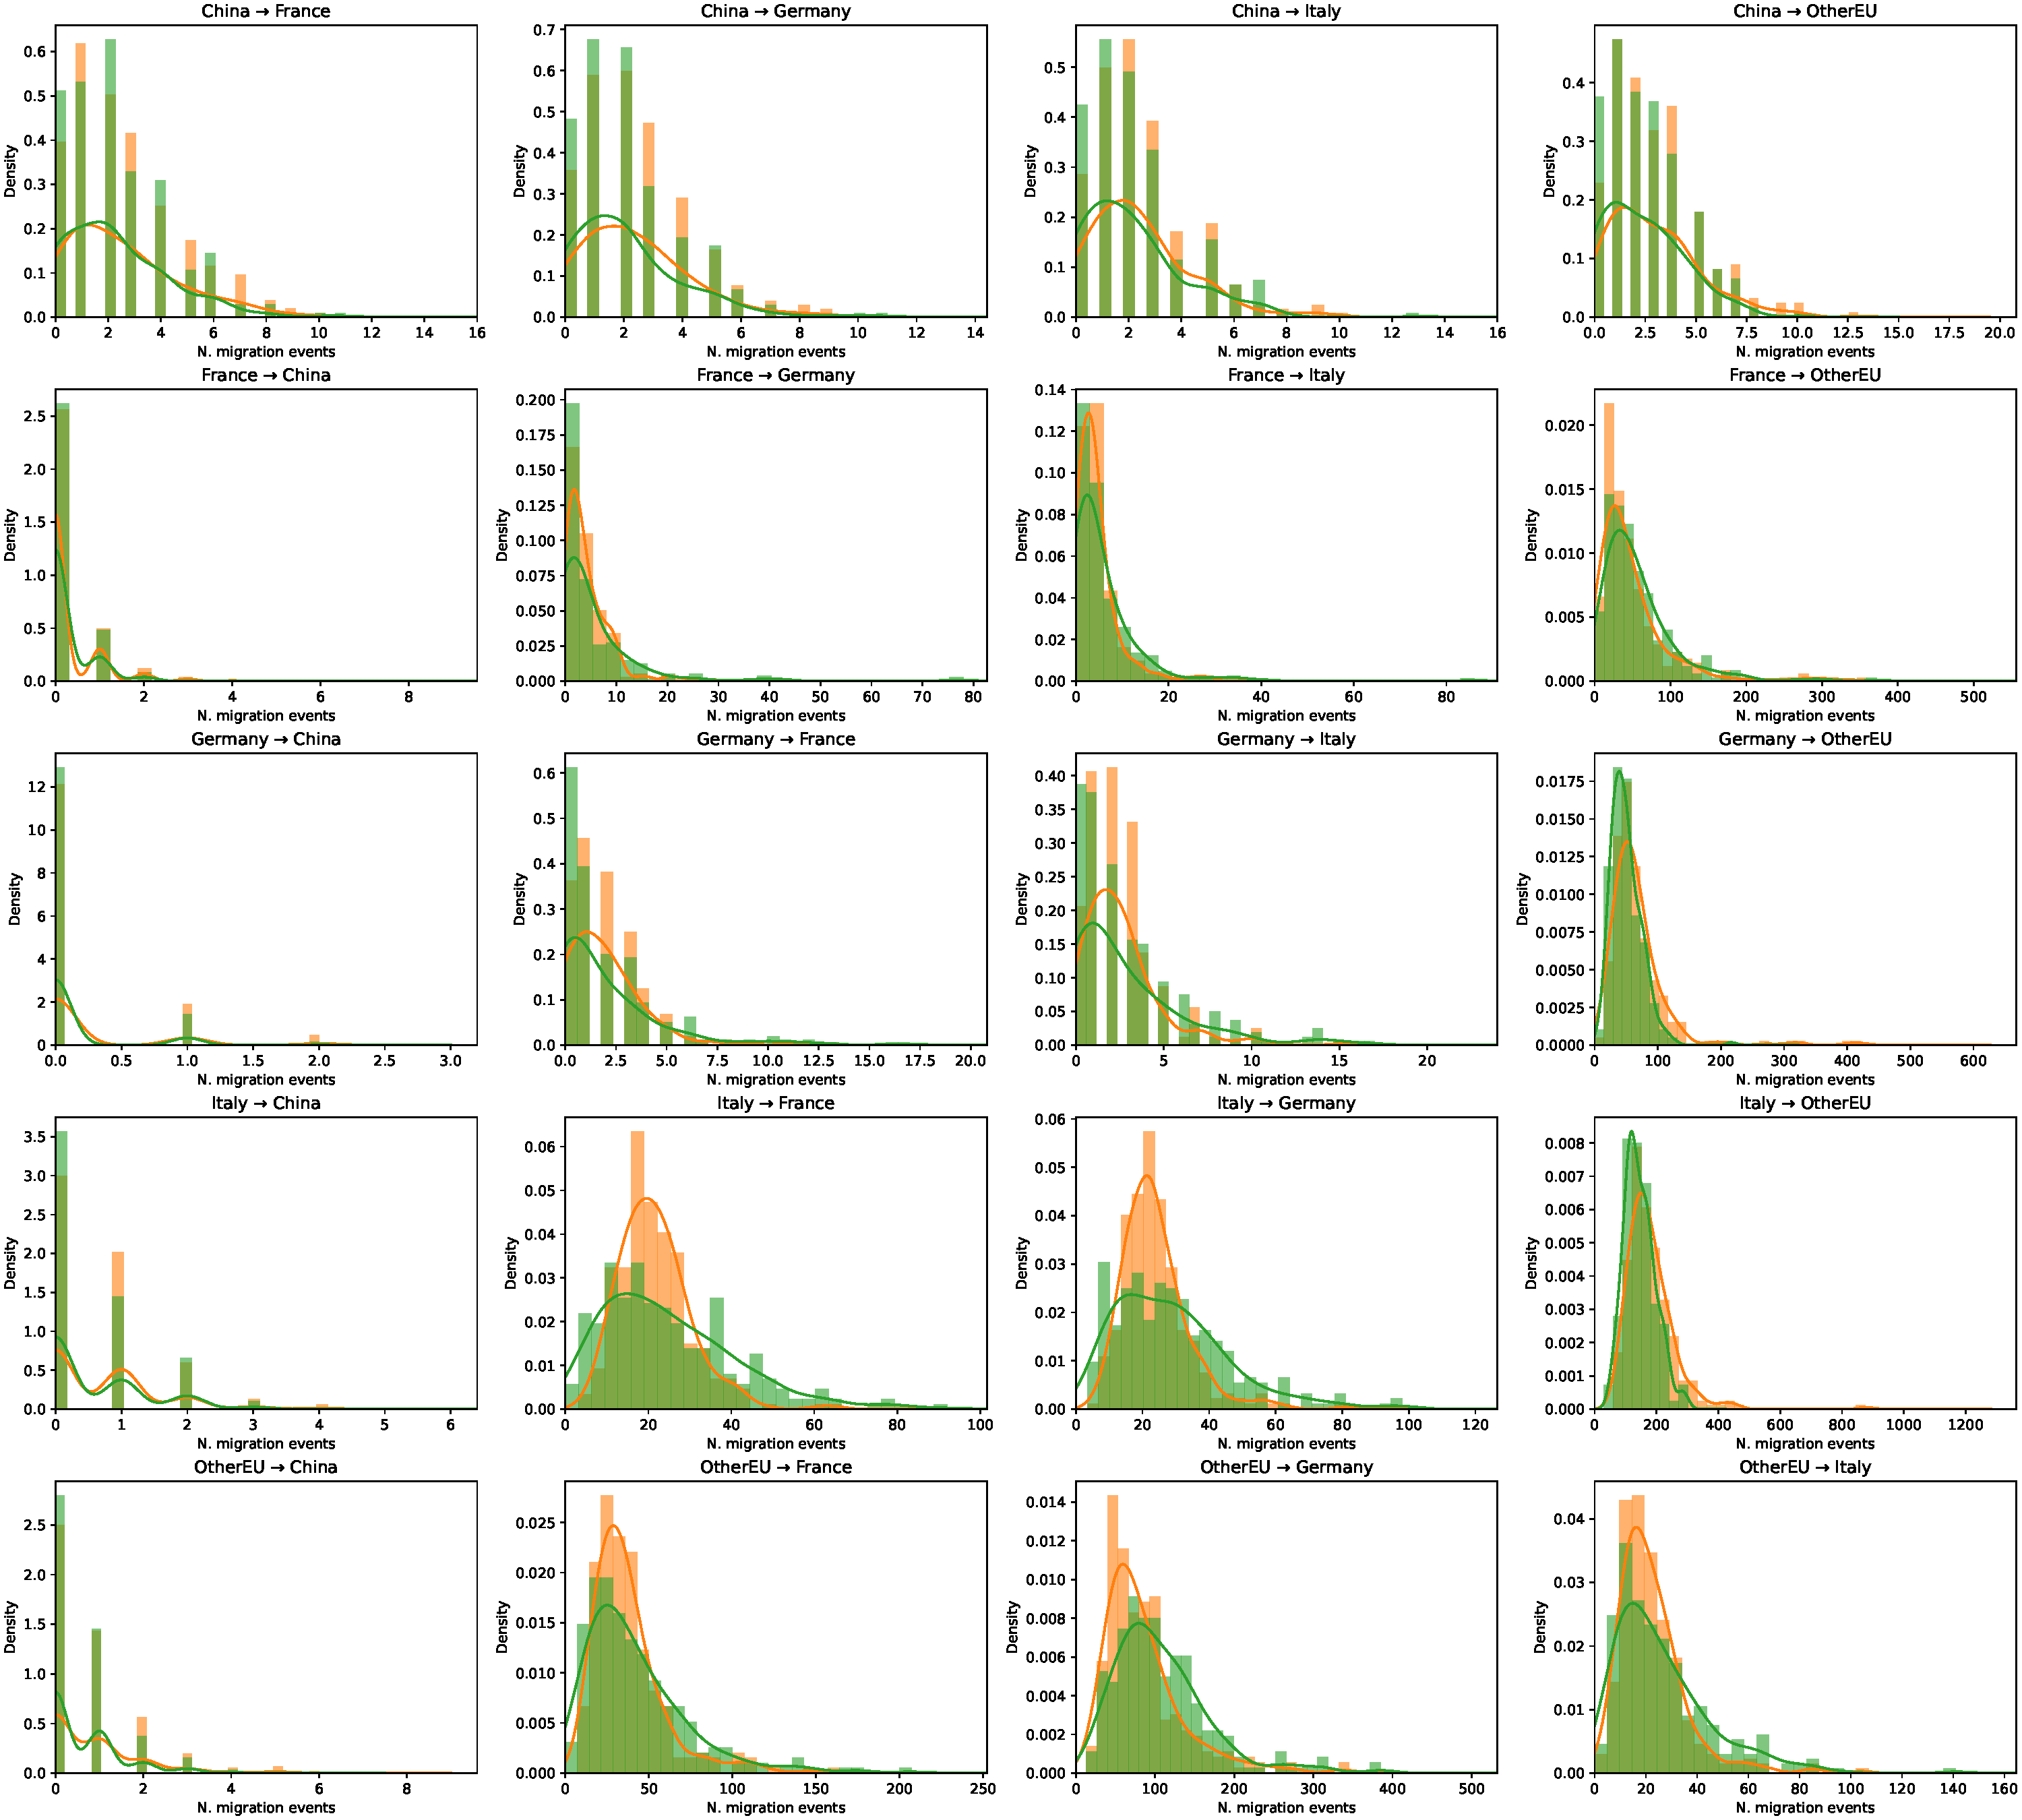
\includegraphics[width=1\textwidth]{figures/eucovid/migrations/time_bin_2.pdf}
    \caption{Distribution of estimated migration fluxes between countries during the early spread of SARS-CoV-2 in Europe for the period from 16 February 2020 to 8 March 2020.}
    \label{fig:eucovid:migrations:time_bin_2}
\end{figure}
